\documentclass[10pt,a4paper]{beamer}
\usepackage[utf8]{inputenc}
\usepackage[T1]{fontenc}
\usepackage[english]{babel}
% \usepackage{hyperref}
\usepackage{amssymb,amsthm,amsmath,amsfonts}
\usepackage{lmodern}
% \usepackage{units}
% \usepackage{hyperref}
\usepackage{tikz}
% \usepackage{tikzsymbols}
\usetikzlibrary{calc}
\usetikzlibrary{fixedpointarithmetic}
\usepackage{fp}
\usepackage{graphicx}
% \bibliographystyle{plain}
\usepackage{epsfig}
\usepackage{epstopdf}
% \usepackage{makeidx}
% \usepackage{gloss}
\usepackage{algorithmic}
% \usepackage{algorithm}
\usepackage{todonotes}

% \usepackage{xkeyval} 

\def\glossname{Glossaire}
%\bibliographystyle{alpha} % plain-fr si rapport en français

% \usepackage[usenames,dvipsnames]{pstricks}
% \usepackage{epsfig}
% \usepackage{pst-grad} % For gradients}}
% \usepackage{pst-plot}



\theoremstyle{plain}
\newtheorem{thm}{Théorème}[part]
\theoremstyle{definition} 
\newtheorem{lem}[thm]{Lemme}
\theoremstyle{definition} 
\newtheorem{cor}[thm]{Corollaire}
\theoremstyle{definition} 
\newtheorem{prop}[thm]{Proposition}
\theoremstyle{definition} 
\newtheorem{defi}[thm]{Définition}
\theoremstyle{remark} 
\newtheorem{rem}[thm]{Remaque}
\theoremstyle{remark} 
\newtheorem{exe}[thm]{Exemple}
\theoremstyle{definition}
\newtheorem{nota}[thm]{Notation}

\useoutertheme{split}
\useinnertheme{rounded}
\usecolortheme{whale}
\usecolortheme{orchid}
\usecolortheme[named=blue]{structure}
\makeatletter

\setbeamertemplate{headline}{%
%  \begin{beamercolorbox}[wd=\paperwidth,ht=3pt]{logo in head}%
%    This is cut by Uni-KL projector
%  \end{beamercolorbox}
  \leavevmode \@tempdimb=2.4375ex%
  \ifnum\beamer@subsectionmax<\beamer@sectionmax%
    \multiply\@tempdimb by\beamer@sectionmax%
  \else%
    \multiply\@tempdimb by\beamer@subsectionmax%
  \fi%
  \ifdim\@tempdimb>0pt%
    \advance\@tempdimb by 1.825ex%
    \begin{beamercolorbox}[wd=.5\paperwidth,ht=\@tempdimb]{section in head/foot}%
      \vbox to\@tempdimb{\vfil\insertsectionnavigation{.5\paperwidth}\vfil}%
    \end{beamercolorbox}%
    \begin{beamercolorbox}[wd=.5\paperwidth,ht=\@tempdimb]{logo in head}%
    \vbox to\@tempdimb{\vfil \hbox to .5\paperwidth{\hfill
    
\includegraphics[scale=0.5]{Images/Logo_Ecole_polytechnique_horizontal_300dpi.jpg} \hfill
  
\includegraphics[height=8mm]{Images/uvsq-logo-cmjn.jpg}\hskip 8mm}\vfil}%
    \end{beamercolorbox}%
  \fi%
}
\setbeamertemplate{footline}{%
  \leavevmode%
  \hbox{\begin{beamercolorbox}[wd=.5\paperwidth,ht=2.5ex,dp=1.125ex,leftskip=.3cm plus1fill,rightskip=.3cm]{author in head/foot}%
    \usebeamerfont{author in head/foot}\insertshortauthor
  \end{beamercolorbox}%
  \begin{beamercolorbox}[wd=.5\paperwidth,ht=2.5ex,dp=1.125ex,leftskip=.3cm,rightskip=.3cm plus1fil]{title in head/foot}%
    \usebeamerfont{title in head/foot}\insertshorttitle \hfill
    \insertframenumber/\inserttotalframenumber
  \end{beamercolorbox}}%
  \vskip0pt%
}
\newcommand{\backupbegin}{ \newcounter{framenumberappendix} \setcounter{framenumberappendix}{\value{framenumber}} \setbeamertemplate{footline}{} } \newcommand{\backupend}{ \addtocounter{framenumberappendix}{-\value{framenumber}} \addtocounter{framenumber}{\value{framenumberappendix}} \setbeamertemplate{footline}{ \vspace{-1cm}\small{\insertframenumber/\inserttotalframenumber} } }

\makeatother
\definecolor{uvsqvert}{RGB}{91,172,41}
\definecolor{uvsqbleu}{RGB}{15,152,209}
% \setbeamercolor{section in head/foot}{fg=black,bg=uvsqvert}
% \setbeamercolor{subsection in head/foot}{fg=black,bg=uvsqvert!80}
\setbeamercolor{logo in head}{fg=black,bg=white}
% \def\insertsubsectionnavigation#1{\hbox to #1{%
%   \hfill 
\includegraphics[height=8mm]{Images/uvsq-logo-cmjn.jpg}}}
\definecolor{pacificcream}{cmyk}{.05,.05,.15,0}


\setbeamerfont{block title}{size={}}
\beamertemplatenavigationsymbolsempty

\newcommand{\orangebox}[2]{
\setbeamercolor{uppercol}{fg=white,bg=orange}
\setbeamercolor{lowercol}{fg=black,bg=pacificcream}

\begin{beamerboxesrounded}[upper=uppercol,lower=lowercol,shadow=true]{
#1 }  #2
\end{beamerboxesrounded} }

\newcommand{\bluebox}[2]{
\setbeamercolor{upperblue}{fg=white,bg=blue}
\setbeamercolor{lowercol}{fg=black,bg=pacificcream}

\begin{beamerboxesrounded}[upper=upperblue,lower=lowercol,shadow=true]{
#1 }  #2
\end{beamerboxesrounded} }

\newenvironment{orangeitemize}{\setbeamertemplate{itemize item}{$\bullet$}\begin{itemize}}{\end{itemize}}
\newenvironment{grassgreenitemize}{\setbeamertemplate{itemize item}{\textcolor{grassgreen}{$\bullet$}} \begin{itemize}}{\end{itemize}}
\newenvironment{blackitemize}{\setbeamertemplate{itemize item}{\textcolor{black}{$\bullet$}} \begin{itemize}}{\end{itemize}}


% \logo{
\includegraphics[height=8mm]{Images/uvsq-logo-cmjn.jpg}} 
% \addtobeamertemplate{footline}{\hfill\insertframenumber/ \inserttotalframenumber \hspace{2em}\null}

\def\algorithmicrequire{\textbf{Entrée:}}
\def\algorithmicensure{\textbf{Sortie:}}

%\DeclareMathOperator{\ker}{ker}

\def\red#1{\textcolor{red}{#1}}
\def\blu#1{\textcolor{blue}{#1}}

\tikzset{position/.style args={#1:#2 from #3}{%
  at=(#3.#1),anchor=#1+180,shift=(#1:#2)}}%
\tikzstyle{lambda}=[very thick,draw=blue,->]
\tikzstyle{mu}=[very thick,draw=red,->]

\begin{document}

\author{
\href{http://www.prism.uvsq.fr/~huc/}{Cyril Hugounenq}
}
%\title[Structure of $\ell$-isogeny volcanoes applied to Couveignes' algorithm]{Structure of $\ell$-isogeny volcanoes applied to Couveignes' algorithm}
\title[Volcans et calculs d'isogénies]{
Volcans et calculs d'isogénies}
\institute{Université de Versailles Saint-Quentin-en-Yvelines}
\date{25 Septembre, 2017}


\begin{frame}
\titlepage

\hfill

\includegraphics[scale=0.6]{Images/Logo_Ecole_polytechnique_horizontal_300dpi.jpg} \hfill

\includegraphics[scale=0.1]{Images/digiteo.jpg}\hfill

\includegraphics[height=10mm]{Images/uvsq-logo-cmjn.jpg}
\end{frame}
%\maketitle
%faire un plan
%faire un rappel sur les courbes elliptiques

\begin{frame}
\frametitle{Intérêts de la cryptographie}
\includegraphics[scale=0.5]{Images/wireshark_threatening_amazon.pdf} 
\end{frame}

\begin{frame}
\frametitle{Intérêts de la cryptographie}
\includegraphics[scale=0.5]{Images/https_protecting_amazon.pdf} 
\end{frame}

\begin{frame}
\frametitle{Intérêts cryptographiques des isogénies}
%We focus on one specific subproblem in the Schoof-Elkies-Atkin point counting  algorithm:
%\medskip

%\bluebox{Disclaimer:}{This is \textbf{not} the dominant step in SEA.}
Les isogénies, à l'image des courbes elliptiques sur les corps finis, ont de nombreuses 
applications en cryptographie: 
\begin{itemize}
\item l'algorithme de Schoof-Elkies-Atkin: algorithme de comptage de points
d'une courbe elliptique, nécessaire pour l'évaluation de la sécurité 
cryptographique d'une courbe elliptique;
\pause
\item cryptanalyse de la cryptographie à l'aide de courbes elliptiques: [Gaudry,~Hess,~Smart '02], [Galbraith,~Hess,~Smart '02];
\pause
\item construction de schéma cryptographique à trappe: [Teske~'06];
\pause
\item construction de fonctions de hachage: [Charles,~Goren,~Lauter '09];
\pause
\item construction de schémas cryptographiques post-quantiques: [Rostovtsev,~Stolbunov~'06], [De~Feo,~Jao,~Pl\^ut~'11].
\end{itemize}
%Probleme du logarithme discret...
\end{frame}

\begin{frame}
\frametitle{Sommaire}
\tableofcontents
\end{frame}

%%%%%%%%%%%%%%%%%%%%%%%%%%%%%%%%%%%%%%%%%%%%%%%%%%%%%%%%%%%%
%%%%%%%%%%%%%%%%%%%%%%%%%%%%%%%%%%%%%%%%%%%%%%%%%%%%%%%%%%%%
\section{Isogénies}
%parler aussi de la cryptographie sur les courbes elliptiques

\begin{frame}
\frametitle{Courbe elliptique }

\begin{defi}[Courbe Elliptique]
Soit $\mathbb{K}$ un corps de caractéristique différente de $2$ et $3$, une courbe elliptique $E$ peut être définie à l'aide d'une équation de Weierstrass: 
%la variété projective associée à l'équation
\begin{equation*}
\label{eq:weierstrass-proj}
E:=\{ (X,Y) \in \overline{\mathbb{K}} , Y^2=X^3+AX+B \} \cup 0_E
\end{equation*}
avec $A,B$ des éléments de $\mathbb{K}$. $0_E$ est appelé le \emph{point à l'infini}. 
%Dès lors que $a_4,a_6$ appartiennent à $\mathbb{K}$ alors la courbe est dite
%définie sur $\mathbb{K}$.
\end{defi}
%Partir directement en coordonnées projectives .
%Faire un dessin de courbe elliptique

\begin{figure}
\begin{center}

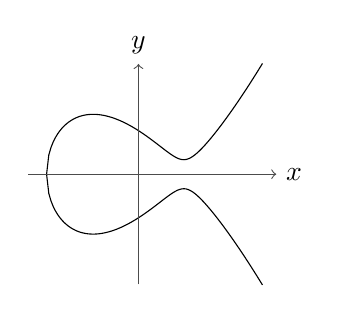
\begin{tikzpicture}[scale=0.35,domain=-10/3:4.5,samples=100,yscale=1/2]
          \begin{scope}[fixed point arithmetic]
            
            \draw plot (\x,{sqrt(\x*\x*\x+(3-100/9)*\x+10)});
            \draw plot (\x,{-sqrt(\x*\x*\x+(3-100/9)*\x+10)});
			\draw[->,color=black!70!white] (-4,0) -- (5,0);
			\draw (5,0) node[right] {$x$};
			\draw [->,color=black!70!white] (0,-8) -- (0,8);
			\draw (0,8) node[above] {$y$};
          \end{scope}
\end{tikzpicture}
\end{center}
%\caption{Représentation d'une courbe elliptique}
\end{figure}
\end{frame}
%%%%%%%%%%%%%%%%%%%%%%%%%%%%%%%%%%%%%%%%%%%%%%%%%%%%%%%%%%%%%
\begin{frame}
\frametitle{Loi de groupe sur une courbe elliptique}

\begin{figure}
\begin{center}

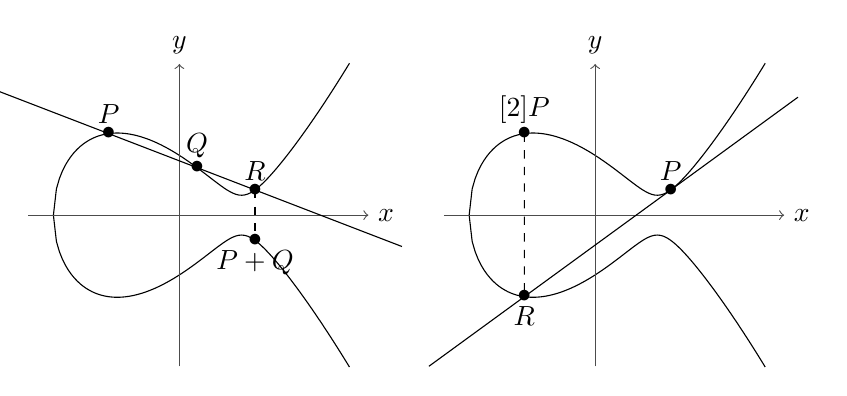
\begin{tikzpicture}[scale=0.480,domain=-10/3:4.5,samples=100,yscale=1/2]
          \begin{scope}[fixed point arithmetic]
            \begin{scope}[fixed point arithmetic]
              \coordinate (Q) at (2, -4/3) {};
              \coordinate (-Q) at (2, 4/3) {};
              \coordinate (-2Q) at (-1079/576, 59653/13824);
              \coordinate (3Q) at (2319138/4977361, 27920423524/11104492391);
            \end{scope}

            \draw plot (\x,{sqrt(\x*\x*\x+(3-100/9)*\x+10)});
            \draw plot (\x,{-sqrt(\x*\x*\x+(3-100/9)*\x+10)});
			\draw[->,color=black!70!white] (-4,0) -- (5,0);
			\draw (5,0) node[right] {$x$};
			\draw [->,color=black!70!white] (0,-8) -- (0,8);
			\draw (0,8) node[above] {$y$};			
			
            \draw[shorten >=-2cm, shorten <=-2cm] (-2Q) -- (-Q);
            \draw[dashed] (-Q) -- (Q);

%            \begin{scope}[/dot/.style={draw,circle,inner sep=1pt,fill},
%              every label/.style={inner sep=5pt,font=\scriptsize}]
%              \draw (-2Q) node[/dot,label=$P$] {}
%               (3Q) node[/dot,label=$Q$] (G) {}
%              (-Q) node[/dot,label=$R$] {};
%              \draw[label position=right,label distance=5pt] (Q) node[/dot,label=$P+Q$] {};
%            \end{scope}
            \draw (-2Q) node{$\bullet$};
            \draw (-2Q) node[above]{$P$};
            \draw (3Q) node{$\bullet$};
            \draw (3Q) node[above]{$Q$};
            \draw (-Q) node{$\bullet$};
            \draw (-Q) node[above]{$R$};
            \draw (Q) node{$\bullet$};
            \draw (Q) node[below]{$P+Q$};
          \end{scope}

          \begin{scope}[xshift=11cm,fixed point arithmetic]
            \draw plot (\x,{sqrt(\x*\x*\x+(3-100/9)*\x+10)});
            \draw plot (\x,{-sqrt(\x*\x*\x+(3-100/9)*\x+10)});
			\draw[->,color=black!70!white] (-4,0) -- (5,0);%axe x
			\draw (5,0) node[right] {$x$};
			\draw [->,color=black!70!white] (0,-8) -- (0,8);%axe y
			\draw (0,8) node[above] {$y$};		
		
            \begin{scope}[fixed point arithmetic]
              \coordinate (-Q) at (2, 4/3) {};
              \coordinate (-2Q) at (-1079/576, 59653/13824);
              \path let \p1 = (-2Q) in coordinate (2Q) at (\x1,-\y1);
            \end{scope}

            \draw[shorten >=-1.5cm, shorten <=-2cm] (-Q) -- (2Q);
            \draw[dashed] (-2Q) -- (2Q);

%            \begin{scope}[/dot/.style={draw,circle,inner sep=1pt,fill},
%              every label/.style={inner sep=5pt,font=\scriptsize}]
%              \draw (-Q) node[/dot] {$P$}
%              (-2Q) node[/dot] (G) {$[2]P$};
%              \draw[label position=below] (2Q) node[/dot] {$R$};
%            \end{scope}
            
            \draw (-Q) node{$\bullet$};
            \draw (-Q) node[above]{$P$};
            \draw (-2Q) node{$\bullet$};
            \draw (-2Q) node[above]{$[2]P$};
            \draw (2Q) node{$\bullet$};
            \draw (2Q) node[below]{$R$};
%			 \begin{scope}[/dot/.style={draw,circle,inner sep=1pt,fill},
%              every label/.style={inner sep=5pt,font=\scriptsize}]
%              \draw (-2Q) node[/dot,label=$P$] {}
%               (3Q) node[/dot,label=$Q$] (G) {}
%              (-Q) node[/dot,label=$R$] {};
%              \draw[label position=right,label distance=5pt] (Q) node[/dot,label=$P+Q$] {};
%            \end{scope}
%          \end{scope}            
            
          \end{scope}
        \end{tikzpicture}

\end{center}
\end{figure}


\begin{prop}
L'ensemble des points d'une courbe elliptique forme un groupe abélien pour la loi additive d'élément neutre $0_E$.
\end{prop}


\end{frame}

%%%%%%%%%%%%%%%%%%%%%%%%%%%%%%%%%%%%%%%%%%%%%%%%%%%%%%%%%%%%%

\begin{frame}
\bluebox{Multiplication scalaire}{On définit alors pour une courbe elliptique 
$E$ et un entier $n$:
\begin{align*}
[n] \;:\; E & \to E\\
P & \mapsto [n] P
\end{align*}}

\hfill

%\vspace{-1mm}

\bluebox{Points de torsion}{
Soit $E$ une courbe elliptique définie sur un corps fini $\mathbb{F}_q$,
et un entier $n$.
\vspace{-1.5mm}
\[E[n]= \{ P \in E(\bar{\mathbb{F}}_q) , [n]P=0_E \} \]
}
\medskip
\bluebox{Polynômes de $n$-division}
{Pour toute courbe elliptique $E$ et tout entier $n$ il existe un polynôme $\omega_n$ tel que les abscisses des points de $n$-torsion soient les racines de ce polynôme.}
%\bluebox{Problème du logarithme discret sur une courbe elliptique $E$}
%{
%\begin{algorithmic}[1]
%\REQUIRE $P \in E$ le générateur du groupe $G:=\langle P \rangle$, $Q=[x]P \in G$;
%\ENSURE $x$.
%\end{algorithmic}
%}
%Il manque un lien avec la suite..
%Dire que c'est donc intéressant de se pencher sur des applications qui permettent de conserver cette propriété....
\end{frame}


%%%%%%%%%%%%%%%%%%%%%%%%%%%%%%%%%%%%%%%%%%%%%%%%%%%%%%%%%%%%%
%%%%%%%%%%%%%%%%%%%%%%%%%%%%%%%%%%%%%%%%%%%%%%%%%%%%%%%%%%%%%


\begin{frame}
\frametitle{Isogénies}
\bluebox{Isogénies}{
\begin{itemize}
\item $E$ et $E'$ deux courbes elliptiques, une isogénie est un morphisme surjectif $\phi: E \rightarrow E'$ tel que $\phi(0_{E})=0_{E'}$. Les isogénies sont
\begin{itemize}
 \item des morphismes de groupe (avec un noyau fini),
 \item des fonctions algébriques (de degré fini).
\end{itemize}
 
\item  Si l'isogénie est de degré $\ell$, nous l'appelons \emph{$\ell$-isogénie},

\item Deux courbes $E$ et $E'$ sont dites \emph{$\ell$-isogènes} si il existe une $\ell$-isogénie qui les relie.

%\item Dans cet exposé: seulement des isogénies \emph{rationnelles} (i.e. invariantes sous l'action de groupe de Galois).

%\item We say that $E$ and $E'$ are isogenous if there exist an isogeny $\phi$ between the two curves.

%\item Moreover if the isogeny $\phi$ is $\textbf{separable}$ then we have $\deg \phi = | \ker(\phi) |$ and if $\ell= \deg \phi $ then we say that the curves $E$ and $E'$ are $\ell$-isogenous.
\end{itemize}
}

% \begin{thm} 
% Let $G\subset E$ be a subgroup of points of order $\ell$. There is an isogeny $\phi:E\to E'$ of degree $\ell$ such that $\ker\phi = G$.
% \end{thm}

% For \emph{separable} isogenies, this defines a bijection between isogenies and finite subgroups.

\textbf{Exemple:}
Soit $\ell$ un entier, l'application \emph{multiplication scalaire}
\begin{align*}
[\ell] \;:\; E &\to E\\
P &\mapsto [\ell] P
\end{align*}
est une isogénie de degré $\ell^2$.

\end{frame}

%%%%%%%%%%%%%%%%%%%%%%%%%%%%%%%%%%%%%%%%%%%%%%%%%%%%%%%%%%%%

\begin{frame}
\frametitle{Isogénie explicite}

\bluebox{Isogénie explicite}{
Les isogénies séparables de degré $\ell$ sont représentables par des fonctions
rationnelles sous forme de Weierstrass
%\[
%\left( x ,y \right) \mapsto \left( \frac{n(x)=45x^9+67x^7+57x^6+97x^5+7+100x^2+78x+67}{d(x)(x^4+51x^2+67x+61)^2}, y\left(\frac{n(x)}{d(x)\right)^'} \right)
%\]
\vspace{-1mm}
\[
\left( x,y \right) \mapsto \left(\frac{n(x)}{d(x)}, cy \left( \frac{n(x)}{d(x)} \right)' \right)
\]
avec $n(x)$ un polynôme de degré $\ell$ et $d(x)$ un polynôme de degré $\ell-1$.
}

%\begin{exe} 
%$E$ an elliptic curve defined over $\mathbb{F}_q$, then we define an $\ell$-isogeny by a point: $P$ of order $\ell$
%\[ \phi: E \rightarrow E/ \left\langle P \right\rangle \]
%\end{exe}

\bluebox{Formules de V\'elu}{
La connaissance du noyau de l'isogénie $\phi$ permet d'expliciter celle-ci
%From the knowledge of its kernel we can explicitly write down the isogeny:
\begin{itemize}
    \item Soit $G=\ker\phi$, alors $\displaystyle d(X)=\prod_{P \in G\setminus\{0_E\}}(X-x(P))$;
    \item Formules de V\'elu : à partir de $d(X)$ on déduit $n(X)/d(X)$;
    %\item Complexity quasi-linear in $\ell = \#G$.
\end{itemize}
}

\end{frame}

%%%%%%%%%%%%%%%%%%%%%%%%%%%%%%%%%%%%%%%%%%%%%%%%%%%%%%%%%%%%
%
%\begin{frame}
%\frametitle{Motivation}
%%We focus on one specific subproblem in the Schoof-Elkies-Atkin point counting  algorithm:
%%\medskip
%\bluebox{Explicit isogeny computation problem}
%{
% Let $\mathbb{F}_q$ be a finite field of characteristic $p$. 
% Given $E$, $E'$   two $r$-isogenous elliptic curves defined over $\mathbb{F}_q$,
% compute an $r$-isogeny $\phi:E\to E'$.
%}
%\medskip
%
%%\bluebox{Disclaimer:}{This is \textbf{not} the dominant step in SEA.}
%
%Applications:
%\begin{itemize}
%\item Schoof-Elkies-Atkin point counting algorithm,
%\item ECC cryptanalysis: [Gaudry,~Hess,~Smart '02],
%\item Hash functions: [Charles,~Goren,~Lauter '07],
%\item Trapdoors: [Teske~'06],
%\item Post quantum cryptography: [Rotostev,~Stolbunov~'06], [De~Feo,~Jao,~Pl\^ut~'11].
%\end{itemize}
%
%\end{frame}
%
%%%%%%%%%%%%%%%%%%%%%%%%%%%%%%%%%%%%%%%%%%%%%%%%%%%%%%%%%%%%%

\begin{frame}
\frametitle{Endomorphismes d'un courbe elliptique}
\begin{defi}[Endomorphisme]
Un endomorphisme d'une courbe elliptique $E$ est une isogénie $\psi:E \rightarrow E$. L'ensemble des endomorphismes d'une courbe $E$ est noté $\mathrm{End}(E)$.
\end{defi}

\smallskip

\textbf{Exemple:} La multiplication scalaire est un endomorphisme.

\smallskip

\begin{prop}
$\left( \mathrm{End}(E),+,\circ \right)$ est un anneau.
\end{prop}
\end{frame}

\begin{frame}
\frametitle{Frobenius}
\begin{defi}[L'endomorphisme de Frobenius]
$E$ une courbe elliptique ordinaire définie sur $\mathbb{F}_q$. Le morphisme
\[ \pi:(x,y) \mapsto (x^q,y^q)\] est appelé endomorphisme de Frobenius. Il
satisfait une équation quadratique \[ \pi^2 - t \pi + q = 0.\]
\end{defi}

Nous travaillons seulement avec des isogénies rationnelles $\psi:E \to E'$, i.e.
\[
\pi_{E'} \circ \psi =\psi \circ \pi_{E}.
 \]
 
\end{frame}

%%%%%%%%%%%%%%%%%%%%%%%%%%%%%%%%%%%%%%%%%%%%%%%%%%%%%%%%%%%%

%%%%%%%%%%%%%%%%%%%%%%%%%%%%%%%%%%%%%%%%%%%%%%%%%%%%%%%%%%%%
%\section{An $\ell$-adic Couveignes algorithm (special case)}
\begin{frame}
\frametitle{Classification des courbes elliptiques sur un corps fini}
\begin{prop}
Soit $E$ une courbe elliptique définie sur $\mathbb{F}_q$ de caractéristique 
$p$. Soit:
\begin{enumerate}
\item $E[p]=\mathbb{Z}/p\mathbb{Z}$,
\item l'anneau des endomorphismes $\mathrm{End}(E)$ est isomorphe à un ordre dans un corps de nombres quadratique imaginaire noté $K$.
\end{enumerate}
$E$ est alors dite \emph{ordinaire}.

Soit:
\begin{enumerate}
\item $E[p]=\{0_E\}$,
\item l'anneau des endomorphismes $\mathrm{End}(E)$ est isomorphe à un ordre dans une algèbre de quaternions.
\end{enumerate}
$E$ est alors dite \emph{supersingulière}.

\end{prop}

\end{frame}

%%%%%%%%%%%%%%%%%%%%%%%%%%%%%%%%%%%%%%%%%%%%%%%%%%%%%
\begin{frame}
\frametitle{Problème du calcul de l'isogénie explicite}
\bluebox{Problème du calcul de l'isogénie explicite}
{
 Soit $\mathbb{F}_q$ un corps fini de caractéristique $p$. 
 \`A partir de $E$, $E'$  deux courbes elliptiques ordinaires $r$-isogènes définies sur 
 $\mathbb{F}_q$, calculer la $r$-isogénie $\phi:E\to E'$.
}
\medskip 
Celui-ci apparaît dans:
\begin{itemize}
 \item{} l'algorithme SEA; 
 \item{} la cryptanalyse de cryptosystèmes (par exemple [Rostovtsev,~Stolbunov~'06]).
\end{itemize}
%\vspace{-1mm}

\end{frame}
\begin{frame}
\frametitle{Précédents travaux}
%Travailler cette slide...
\begin{itemize}
\item{} [Elkies~'89],[Charlap, Colay, Robbins~'91], [Atkin~'91].
\item{} [Elkies~'92/'98],  %[Charlap, Colay, Robbins '91], 
[Bostan,~Morain,~Salvy,~Schost~'08], [Lercier,~Sirvent~'08], [Lairez,~Vaccon~'16] fonctionne en $\tilde{O}(r \log(p))$ opérations dans $\mathbb{F}_q$. Spécifique au contexte SEA.
\pause
\item{} [Couveignes~'94] en $\tilde{O}(r^3p^{O(1)})$ 
opérations.
\pause
\item{} [Lercier~'97] fonctionne seulement pour $p=2$.
\pause
\item{} [Couveignes~'96], [De Feo~'10] en  $\tilde{O}
(r^2p^{O(1)})$ opérations.
\end{itemize}
\begin{itemize}

%\item[$\rightarrow$] we focus on the medium characteristic case ($n\gg p/\log(p)$),
\pause
\item[$\rightarrow$] Nous voulons modifier l'algorithme de Couveignes~'96 pour 
obtenir un algorithme avec une complexité de  $\tilde{O}(r^2)$ mais sans 
dépendance exponentielle en $\log(p)$.
\end{itemize}
\end{frame}

%%%%%%%%%%%%%%%%%%%%%%%%%%%%%%%%%%%%%%%%%%%%%%%%%%%%%%%%%%%%
\section{Algorithme de Couveignes}
\begin{frame}

Pour les courbes elliptiques \emph{ordinaires}
\vspace{-1.5mm}
\begin{align*}
E[\ell^k]&\simeq\mathbb{Z}/\ell^k\mathbb{Z} \times \mathbb{Z}/\ell^k\mathbb{Z} \quad \textit{avec } \ell \neq p \\
E[p^k]&\simeq\mathbb{Z}/p^k\mathbb{Z}
\end{align*}
\pause
\vspace{-5.1mm}
\bluebox{Algorithme de Couveignes (calcul d'une $r$-isogénie $\phi:E\to E'$)}{
Calcul de $\phi$ par interpolation sur $E[p^k]$:
\begin{itemize}
\item Calcul de générateurs $P,P'$ de $E[p^k],E'[p^k]$;
\item Interpolation de $\phi$, en supposant que l'on a la correspondance $P\mapsto P'$;
\begin{itemize}
 	\item Calcul du polynôme d'interpolation $L$ qui envoie $P \mapsto P'$ \\
	\item Calcul d'une fraction rationnelle $F$ de degrés $(r, r-1)$ \\
	à l'aide d'un algorithme de reconstruction rationnelle; 
	\hfill $\color{blue!50!gray}{\tilde{O}(r)}$
\end{itemize}
\vspace{-1.5mm}
\item Vérification si l'interpolation définit une isogénie.\hfill $\color{blue!50!gray}{\tilde{O}(r)}$;
	\begin{itemize}
	\item Test du degré du dénominateur $d$ de $F$ et de sa décomposition en 
	facteurs carré et si $\omega_{\ell}^2= 0 \bmod d$;
	\end{itemize}
    Si ce n'en est pas une, on remplace $P'$ par un multiple $[a]P'$.
\end{itemize}

}
\end{frame}

%%%%%%%%%%%%%%%%%%%%%%%%%%%%%%%%%%%%%%%%%%%%%%%%%%%%%%%%%%%%

\begin{frame}
\frametitle{Algorithme de Couveignes}
\bluebox{}{ %\cite{DBLP:conf/ants/Couveignes96}}{
\begin{algorithmic}[1]
\REQUIRE $E, E',r$ tels que $E$ et $E'$ soient deux courbes $r$-isogènes sur $\mathbb{F}_{p^n}$ 
\ENSURE $\phi: E \rightarrow E'$ de degré $r$
\end{algorithmic}}

\begin{enumerate}
\item Choix du plus petit entier $k$ tel que $p^{k}>4r$.
\item Calcul des générateurs $P$ de
  $E[p^k]$ et $P'$ de $E'[p^k]$; \hfill $\color{blue!50!gray}{\tilde{O}(r p^{O(1)})}$
\item Calcul de $T=\prod(X-x([u]P))$ avec $1\le u \le \frac{p^k-1}{2}$; \hfill $\color{blue!50!gray}{\tilde{O}(r p^{O(1)})}$
\item Pour tout $a \in \left( \mathbb{Z}/p^k\mathbb{Z}\right)^{\times}$:\hfill $\color{blue!50!gray}{O(r)}$
  \begin{enumerate}
%  \item Calcul et test d'un candidat à l'aide d'un polynôme \\ 
%  d'interpolation $L$ qui envoie $P \mapsto [a]P'$ \hfill 
%  $\color{blue!50!gray}{\tilde{O}(r\ell^{O(1)})}$
  \item Calcul du polynôme d'interpolation 
    $L$ tel que
   $L (x ([u] P)) = x([a\, u\,]P' )$ pour tout
    $u \in \mathbb{Z}/p^k \mathbb{Z}$;
\hfill $\color{blue!50!gray}{\tilde{O}(r p^{O(1)})}$
	%\item Utilisation d'un algorithme de reconstruction rationnelle afin de 
	%calculer une fraction rationnelle $F=L\bmod{T}$ de degrés~$(r, r-1)$;
%\hfill $\tilde{O}(r)$
	\item Calcul d'une fraction rationnelle $F=L\bmod{T}$ de degrés \\
	$(r, r-1)$ et test de celle-ci.
	\hfill $\color{blue!50!gray}{\tilde{O}(r)}$
  \end{enumerate}
\end{enumerate}
%Complexity polynomial in $p$. 
\pause
\bluebox{Objectif} {Remplacer $E[p^k]$ par \boldmath $E[\ell^k]$ \unboldmath pour un petit premier $\ell \neq p$.}
\end{frame}

%%%%%%%%%%%%%%%%%%%%%%%%%%%%%%%%%%%%%%%%%%%%%%%%%%%%%%%%%%%%

\begin{frame}

\frametitle{Un algorithme de Couveignes $\ell$-adique ?}
\bluebox{}{
Notre objectif est de travailler avec \boldmath $E[\ell^k]\simeq \left(\mathbb{Z}/\ell^k \mathbb{Z} \right)^2$ \unboldmath 
%Our goal is to work with \textcolor{red}{$E[\ell^k]= \left(\mathbb{Z}/\ell^k \mathbb{Z} \right)^2$}  
à la place de $E[p^k]$ afin de s'affranchir de la dépendance polynomiale en $p$.
\begin{itemize}

%\item[$\Rightarrow$] main drawback: $E[\ell^{\frac{k}{2}}]=\left(\mathbb{Z}/\ell^{\frac{k}{2}} \mathbb{Z} \right)^2$ thus for two basis $\langle P,Q \rangle=E[\ell^{\frac{k}{2}}]$, $\langle P',Q' \rangle=E'[\ell^{\frac{k}{2}}]$ we have to test $O(\ell^{\frac{4k}{2}})=O(r^2)$ mapping candidates before finding the good one for the interpolation.
\item $E[p^k] = \langle P\rangle\simeq\left(\mathbb{Z}/p^{k} \mathbb{Z}
\right)$ \hfill avec $p^{k} \approx r$
\item $E[\ell^k] = \langle P,Q\rangle\simeq\left(\mathbb{Z}/\ell^{k}
\mathbb{Z} \right) \times \left(\mathbb{Z}/\ell^{k} \mathbb{Z} \right)$
\hfill avec $\color{red} \ell^{2k} \approx r$
\end{itemize}}
\pause
\begin{columns}
\begin{column}{0.48\textwidth}

\bluebox{$p$-adique}{
Soient $\langle P \rangle= E[p^k]$ et \\ $\langle P' \rangle= E'[p^k]$
\[
P \mapsto [a] P'  \qquad a\in(\mathbb{Z}/p^k\mathbb{Z})^*
\]

$\Rightarrow O(r)$ possibilités.
}
\end{column}
\begin{column}{0.55\textwidth}
\bluebox{$\ell$-adique}{
Soient $ \langle P,Q \rangle = E[\ell^k]$ et \\ $\langle P',Q' \rangle = E'[\ell^k]$
\begin{gather*}
\begin{pmatrix}
P\\Q
\end{pmatrix}
\mapsto
\begin{pmatrix}
a & b \\
c & d
\end{pmatrix}
\begin{pmatrix}
P'\\Q'
\end{pmatrix}
\\[1ex]
\text{avec $\left(\begin{smallmatrix}a&b\\c&d\end{smallmatrix}\right)\in \mathsf{GL}_2(\mathbb{Z}/\ell^k\mathbb{Z})$ inversible}.
\end{gather*}
$\Rightarrow O(r^2)$ possibilités.
}
\end{column}
\end{columns}

%\pause
%\begin{center}
%    Ouch! Can we restrict the choices for $\left(\begin{smallmatrix}a&b\\c&d\end{smallmatrix}\right)$?
%\end{center}

\end{frame}
\section{Graphes d'isogénies}

%%%%%%%%%%%%%%%%%%%%%%%%%%%%%%%%%%%%%%%%%%%%%%%%%%%%%%%%


%\begin{frame}
%%\section{Computation of endomorphism rings}
%\frametitle{Computation of endomorphism rings}
%
%
%\begin{defi}
%Une courbe elliptique $E$ est dite à multiplication complexe si $\mathrm{End}(E)$ n'est pas réduit à $\mathbb{Z}$.
%\end{defi}
%On a le résultat suivant sur la structure de $\mathrm{End}(E)$.
%
%\end{frame}

\begin{frame}

\begin{prop}
Soit $E$ une courbe elliptique ordinaire, alors 
\[
\mathbb{Z} \left[ \pi \right] \subset \mathcal{O} \subset \mathcal{O}_K
\] 
avec $\mathcal{O}_K$ l'anneau des entiers de $K$ et $\mathcal{O}$ l'ordre 
associé à isomorphisme près à $\mathrm{End}(E)$. %le corps de nombre quadratique imaginaire tel que $\mathcal{O} \subset K$
\end{prop}

\begin{defi}[Discriminant]
On note $d_{\pi}$ (resp. $d_K$) le discriminant de l'ordre $\mathbb{Z}\left[ \pi \right]$ (resp. $\mathcal{O}_K$).
\end{defi}

\begin{defi}[Conducteur]
On note $g=[\mathcal{O}_K:\mathbb{Z}[\pi]]$ le conducteur de $\mathbb{Z}[\pi]$. %et $f$ le conducteur de $[\mathcal{O}_K:\mathcal{O}]$.
\end{defi}

En particulier: $d_{\pi}=g^2d_K$

\end{frame}
%%%%%%%%%%%%%%%%%%%%%%%%%%%%%%%%%%%%%%%%%%%%%%%%%%%%%%%%%%%%

\begin{frame}
\frametitle{Exemple illustratif de graphe d'isogénies}
\begin{figure}
\begin{center}
\begin{tikzpicture}[scale=0.545]
\coordinate (A) at (0,-7.528648782);
\coordinate (B) at (0,-3.75);
\coordinate (C) at (0,0);
\draw (A) node[left]{
$
\mathbb{Z}[\pi]=\mathbb{Z}~+~\ell^2~\mathcal{O}_K 
$
} ;
\draw (A) node{$\bullet$};
\draw (B) node[left]{$\mathbb{Z} + \ell \mathcal{O}_K$} node{$\bullet$};
\draw (C) node[left]{$\mathcal{O}_K$} node{$\bullet$};
\draw (A)--(B)node[midway,left] {$\ell$};
\draw (B)--(C) node[midway,left] {$\ell$};
	\begin{scope}[xshift=6.0cm]
		\node (A) at (-3,0) {$\bullet$};
		\node (B) at (3,0) {$\bullet$};
		\node (C) at (270:1.2) {$\bullet$};
		\node (D) at (90:1.5) {};
		%\draw[-] (A.center) to[bend right=25] (C.center);
		\draw[-,dashed] (A.center) to[bend left=40] (B.center);
		%\draw[-] (B.center) to[bend left=25] (C.center);
		%\draw[-,dashed] (B.center) to[bend right] (D.center);
		\draw[-] (A.center) to[bend right=40] (B.center);
			\begin{scope}[xshift=-3cm]
			\coordinate (A) at (0,0);
			\coordinate (C) at (270:3.75);
			\coordinate (CA) at (265:7.5);
			\coordinate (CB) at (275:7.5);
			\draw (C)--(CA);
			\draw (C)--(CB);
			\draw (CA) node{$\bullet$};
			\draw (CB) node{$\bullet$};
			\draw (A) node{$\bullet$};
			\draw (C) node{$\bullet$};
			\draw (A)--(C);
			\end{scope}
			\begin{scope}[xshift=3cm]
			\coordinate (A) at (0,0);
			\coordinate (C) at (270:3.75);
			\coordinate (CA) at (265:7.5);
			\coordinate (CB) at (275:7.5);
			\draw (C)--(CA);
			\draw (C)--(CB);
			\draw (CA) node{$\bullet$};
			\draw (CB) node{$\bullet$};
			\draw (A) node{$\bullet$};
			\draw (C) node{$\bullet$};
			\draw (A)--(C);
			\end{scope}
			\begin{scope}[yshift=-1.2cm]
			\coordinate (A) at (0,0);
			\coordinate (C) at (270:3.75);
			\coordinate (CA) at (265:7.5);
			\coordinate (CB) at (275:7.5);
			\draw (C)--(CA);
			\draw (C)--(CB);
			\draw (CA) node{$\bullet$};
			\draw (CB) node{$\bullet$};
			\draw (A) node{$\bullet$};
			\draw (C) node{$\bullet$};
			\draw (A)--(C);   
			\end{scope}
	\end{scope}
%faire des fleches courbees avec les indices \ell et \ell^2


\end{tikzpicture}
\end{center}		
\end{figure}

\end{frame}


%%%%%%%%%%%%%%%%%%%%%%%%%%%%%%%%%%%%%%%%%%%%%%%%%%%%%%%%%%%%
\begin{frame}
\frametitle{Illustration des différents types d'isogénies}
%\only<2-4>{
%La notation $\mathcal{O}$ désigne (resp. $\mathcal{O}'$) l'ordre associé à isomorphisme près à l'anneau des endomorphismes de $E$ (resp. $E'$)}
\vspace{-4mm}
\begin{columns}
\begin{column}{4cm}

\begin{lem}[Kohel 1996]
Soient $E$ et $E'$ deux courbes elliptiques définies sur $\mathbb{F}_q$, $\psi :E \rightarrow E'$ une $\ell$-isogénie. Alors $\psi$ est dite
\begin{enumerate}
\item  \textbf<1>{descendante} si $[\mathcal{O} : \mathcal{O}']=\ell$,
\item \textbf<2>{ascendante} si $[\mathcal{O}':\mathcal{O}]=\ell$,
\item \textbf<3>{horizontale} si \\
 $\mathcal{O}=\mathcal{O}'$.
\end{enumerate}
\end{lem}
%\begin{defi}
%The index $f=[\mathcal{O}_K : \mathcal{O}]$ is called the conductor of $\mathcal{O}$.
%\end{defi}
\end{column}


\begin{column}{6cm}
%\includegraphics[scale=.66]{Images/ordres-l.eps}
\begin{figure}
\begin{center}

\begin{tikzpicture}[scale=0.545, xshift=-0.5cm]
	\begin{scope}[xshift=4.4cm]
		\node (A) at (-3,0) {$\bullet$};
		\node (B) at (3,0) {$\bullet$};
		\node (C) at (270:1.2) {$\bullet$};
		\node (D) at (90:1.5) {};
		%\draw[-] (A.center) to[bend right=25] (C.center);
		\draw[-,dashed] (A.center) to[bend left=40] (B.center);
		%\draw[-] (B.center) to[bend left=25] (C.center);
		%\draw[-,dashed] (B.center) to[bend right] (D.center);
		\only<1-2>{
		\draw[-] (A.center) to[bend right=40] (B.center);
		}
		\only<3-3>{
		\draw[-] (C.center) to[bend right=20] (B.center);
		\draw[line width=1.5pt,red,->] (A.center) to[bend right=20] (C.center);
		}
			\begin{scope}[xshift=-3cm]
			\coordinate (A) at (0,0);
			\coordinate (C) at (270:3.75);
			\coordinate (CA) at (265:7.5);
			\coordinate (CB) at (275:7.5);
			\draw (C)--(CA);
			\draw (C)--(CB);
			\draw (CA) node{$\bullet$};
			\draw (CB) node{$\bullet$};
			\draw (A) node{$\bullet$};
			\draw (C) node{$\bullet$};
			\draw (A)--(C);
			\end{scope}
			\begin{scope}[xshift=3cm]
			\coordinate (A) at (0,0);
			\coordinate (C) at (270:3.75);
			\coordinate (CA) at (265:7.5);
			\coordinate (CB) at (275:7.5);
			\draw (C)--(CA);
			\draw (C)--(CB);
			\draw (CA) node{$\bullet$};
			\draw (CB) node{$\bullet$};
			\draw (A) node{$\bullet$};
			\draw (C) node{$\bullet$};
			\draw (A)--(C);
			\end{scope}
			\begin{scope}[yshift=-1.2cm]
			\coordinate (A) at (0,0);
			\coordinate (C) at (270:3.75);
			\coordinate (CA) at (265:7.5);
			\coordinate (CB) at (275:7.5);
			\draw (C)--(CA);
			\draw (C)--(CB);
			\draw (CA) node{$\bullet$};
			\draw (CB) node{$\bullet$};
			\draw (A) node{$\bullet$};
			\draw (C) node{$\bullet$};
			\draw (A)--(C);
            \only<1-1>{
            \draw[line width=1.5pt,red,->] (A)--(C);
            }
            \only<2-2>{
			\draw[line width=1.5pt,red,<-] (A)--(C);            
            }
			\end{scope}
	\end{scope}
%faire des fleches courbees avec les indices \ell et \ell^2


\end{tikzpicture}
\end{center}		
\end{figure}
\end{column}
\end{columns}
\end{frame}


%%%%%%%%%%%%%%%%%%%%%%%%%%%%%%%%%%%%%%%%%%%%%%%%%%%%%%%%%%%%

\begin{frame}
\frametitle{Un guide pour les différents types de volcans}%
\begin{figure}[h]
		\begin{center}
        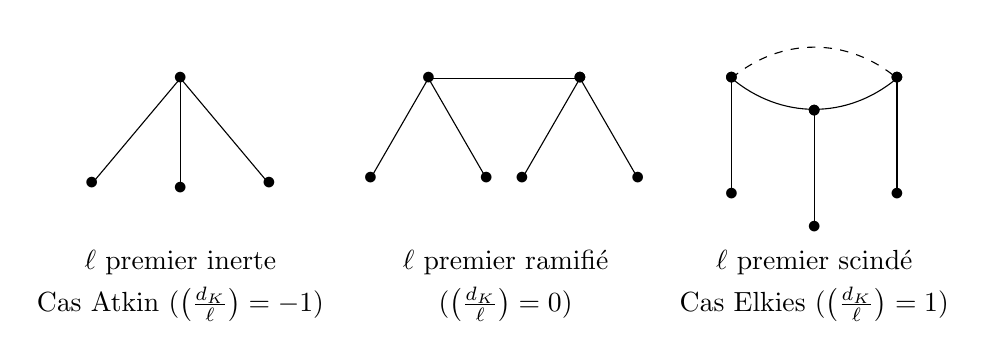
\begin{tikzpicture}[scale=0.35]
        \coordinate (A) at (0,0);
		\coordinate (B) at (230:5);
		\coordinate (C) at (270:4);
		\coordinate (D) at (310:5);
		\draw (A) node{$\bullet$};
		\draw (B) node[fill=white]{$\bullet$};
		\draw (C) node[fill=white]{$\bullet$};
		\draw (D) node[fill=white]{$\bullet$};
		\node at (0,-6.7) {$\ell$ premier inerte};
		\node at (0,-8.2) {Cas Atkin ($\left( \frac{d_{K}}{\ell} \right) = -1$)};
		\draw (A)--(B); 
		\draw (A)--(C);
		\draw (A)--(D);		
		\begin{scope}[xshift=9cm]
		\coordinate (A) at (0,0);
		\coordinate (B) at (5.5,0);
		\coordinate (C) at (240:4.2);
		\coordinate (D) at (300:4.2);
		\draw (A) node[fill=white]{$\bullet$};
		\draw (B) node[fill=white]{$\bullet$};
		\draw (C) node[fill=white]{$\bullet$};
		\draw (D) node[fill=white]{$\bullet$};
		\node at (2.8,-6.7) {$\ell$ premier ramifié};
		\node at (2.8,-8.2) {($\left( \frac{d_{K}}{\ell} \right) = 0$)};
		\draw (A)--(B);
		\draw (A)--(C);
		\draw (A)--(D);
		\end{scope}
		
		\begin{scope}[xshift=14.5cm]
		\coordinate (A) at (0,0);
		\coordinate (C) at (240:4.2);
		\coordinate (D) at (300:4.2);
		\draw (A) node {$\bullet$};
		\draw (C) node {$\bullet$};
		\draw (D) node {$\bullet$};
		\draw (A)--(C);
		\draw (A)--(D);
		\end{scope}
		
		\begin{scope}[xshift=23cm]
		\node (A) at (-3,0) {$\bullet$};
		\node (B) at (3,0) {$\bullet$};
		\node (C) at (270:1.2) {$\bullet$};
		\node (D) at (90:1.5) {};
		\node at (0,-6.7) {$\ell$ premier scindé};
		\node at (0,-8.2) {Cas Elkies ($\left( \frac{d_{K}}{\ell} \right) = 1$)};
		%\draw[-] (A.center) to[bend right=25] (C.center);
		\draw[-,dashed] (A.center) to[bend left=40] (B.center);
		%\draw[-] (B.center) to[bend left=25] (C.center);
		%\draw[-,dashed] (B.center) to[bend right] (D.center);
		\draw[-] (A.center) to[bend right=40] (B.center);
			\begin{scope}[xshift=-3cm]
			\coordinate (A) at (0,0);
			\coordinate (C) at (270:4.2);
			\draw (A) node {$\bullet$};
			\draw (C) node {$\bullet$};
			\draw (A)--(C);
			\end{scope}
			\begin{scope}[xshift=3cm]
			\coordinate (A) at (0,0);
			\coordinate (C) at (270:4.2);
			\draw (A) node {$\bullet$};
			\draw (C) node {$\bullet$};
			\draw (A)--(C);
			\end{scope}
			\begin{scope}[yshift=-1.2cm]
			\coordinate (A) at (0,0);
			\coordinate (C) at (270:4.2);
			\draw (A) node {$\bullet$};
			\draw (C) node {$\bullet$};
			\draw (A)--(C);
			\end{scope}
		\end{scope}
		\end{tikzpicture}
		%\end{center}
		\caption{Les trois formes de volcans de $2$-isogénies }
		
		\end{center} 
		\end{figure}
		Durant le reste de cet exposé nous étudierons le cas Elkies et le cas Atkin.
%\begin{figure}[hbtp]
%\centering
%\includegraphics[scale=0.4]{Images/duo-volcan-wo-label.png}
%\caption{Volcano with one point on the crater, and two points}
%\end{figure}
\end{frame}
%%%%%%%%%%%%%%%%%%%%%%%%%%%%%%%%%%%%%%%%%%%%%%%%%%%%%%%%%%%%

\begin{frame}
\frametitle{Études des différents cas de Couveignes $\ell$-adique}
\vfill
\begin{itemize}
\item Cas Elkies (issu d'un travail conjoint avec \href{http://defeo.lu/}{De Feo}, Plût et \href{https://cs.uwaterloo.ca/~eschost/}{Schost} publié à ANTS XII en 2016)
\begin{itemize}
\vfill
\item Cas Elkies avec hauteur $h=0$;
\vfill
\item Cas Elkies avec hauteur $h \neq 0$;
\end{itemize}
\vfill
\item Cas Atkin
\begin{itemize}
\vfill 
\item Cas Atkin avec hauteur $h=0$;
\vfill
\item Cas Atkin avec hauteur $h \neq 0$;
\end{itemize}
\end{itemize}
\vfill

\end{frame}


%%%%%%%%%%%%%%%%%%%%%%%%%%%%%%%%%%%%%%%%%%%%%%%%%%%%%%%%%%%%%%%%%%%%%%%%

%\begin{frame}
%    \begin{columns}
%        \begin{column}{0.8\textwidth}
%            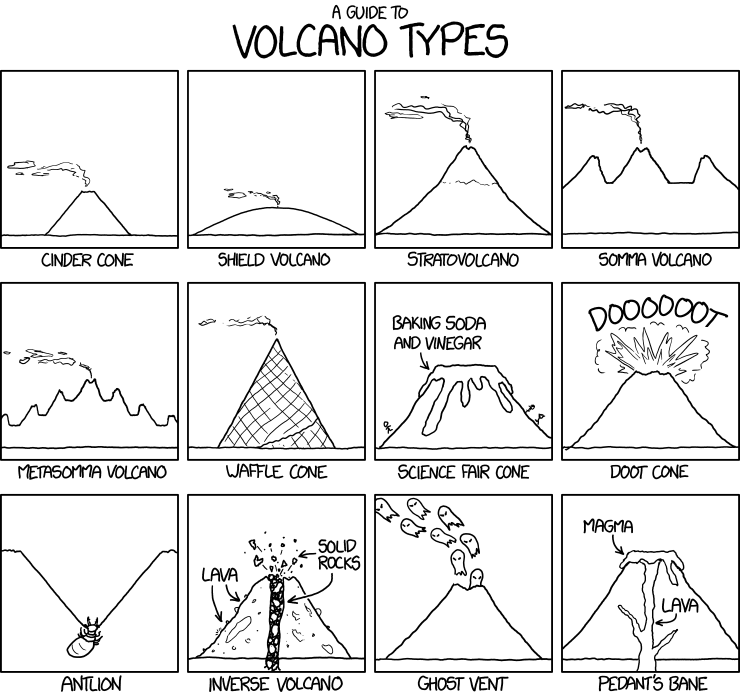
\includegraphics[height=\textheight]{Images/xkcd.png}
%        \end{column}
%        \begin{column}{0.2\textwidth}
%            \href{http://xkcd.com/1714/}{xkcd.com/1714}
%        \end{column}
%    \end{columns}
%\end{frame}

%%%%%%%%%%%%%%%%%%%%%%%%%%%%%%%%%%%%%%%%%%%%%%%%%%%%%%%%%%%%
%%%%%%%%%%%%%%%%%%%%%%%%%%%%%%%%%%%%%%%%%%%%%%%%%%%%%%%%%%%%

\section{Algorithme de Couveignes $\ell$-adique}



\begin{frame}

\vspace{-4mm}
  \begin{center}
    \begin{tabular}{p{13em}p{2em}p{13em}}
Sous-groupe de taille $\ell$  & $\Leftrightarrow$ &     $\ell$-isogénie \pause \\[2mm]
      
    Sous-groupe de taille $\ell$ stable sous l'action de $\pi$   & $\Leftrightarrow$ & $\ell$-isogénie rationnelle 
    \end{tabular}
  \end{center}


\pause
Supposons que $\pi$ se scinde modulo $\ell$:
i.e. son polynôme minimal se factorise comme
\[ (\pi-\red \lambda)(\pi- \blu \mu ) \quad \text{avec} \quad \red \lambda \neq \blu \mu \bmod \ell \]


\pause
\begin{center}
  \begin{tabular}{p{13em}p{2em}p{13em}}
     \raggedright Deux espaces propres de $E[\ell]$:
     \mbox{$\ker(\pi-\red \lambda), \ker( \pi- \blu \mu)$}
     & $\Rightarrow$  
     & \raggedright Deux $\ell$-isogénies rationnelles 
    \mbox{de direction $\red \lambda, \blu \mu $}
  \end{tabular}
\end{center}
%
\bluebox{Graphe d'isogénies}{
\begin{figure}[h]
	\begin{center}
	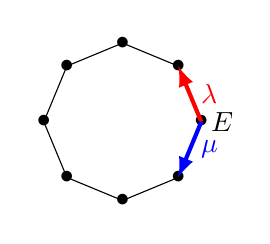
\begin{tikzpicture}[scale=0.20]
	\coordinate (A) at (0:5);
	\coordinate (B) at (45:5);
	\coordinate (C) at (90:5);
	\coordinate (D) at (135:5);
	\coordinate (E) at (180:5);
	\coordinate (F) at (225:5);
	\coordinate (G) at (270:5);
	\coordinate (H) at (315:5);
	\draw (A)--(B)--(C)--(D)--(E)--(F)--(G)--(H)--(A);	
		
	\draw (A) node[right]{$E$};
	\draw (A) node{$\bullet$};
	\draw (B) node{$\bullet$};
	\draw (C) node{$\bullet$};
	\draw (D) node{$\bullet$};
	\draw (E) node{$\bullet$};
	\draw (F) node{$\bullet$};
	\draw (G) node{$\bullet$};
	\draw (H) node{$\bullet$};
	
	\draw[line width=1.5pt,red,-latex] (A)--(B) node[midway,right]{$\color{red} \lambda$};
	\draw[line width=1.5pt,blue,-latex] (A)--(H) node[midway,right]{$\color{blue} \mu$};
		\end{tikzpicture}	
	\end{center}
\end{figure}
}

\end{frame}
%%%%%%%%%%%%%%%%%%%%%%%%%%%%%%%%%%%%%%%%%%%%%%%%%%%%%%%%%%%%

\begin{frame}
  \bluebox{Fait}{
    Soit $\phi$ une $r$-isogénie avec $\ell \nmid r$, alors $\phi$ préserve les
    noyaux des $\ell$-isogénies de \emph{direction} $\red \lambda, \blu \mu $.}

  Pour interpoler $\phi$ sur $E[\ell^k]$, nous voulons calculer deux 
  sous-groupes cycliques de taille $\ell^k$ et de direction $\red \lambda, \blu
  \mu $. 

  \begin{figure}[h]
    \begin{center}
      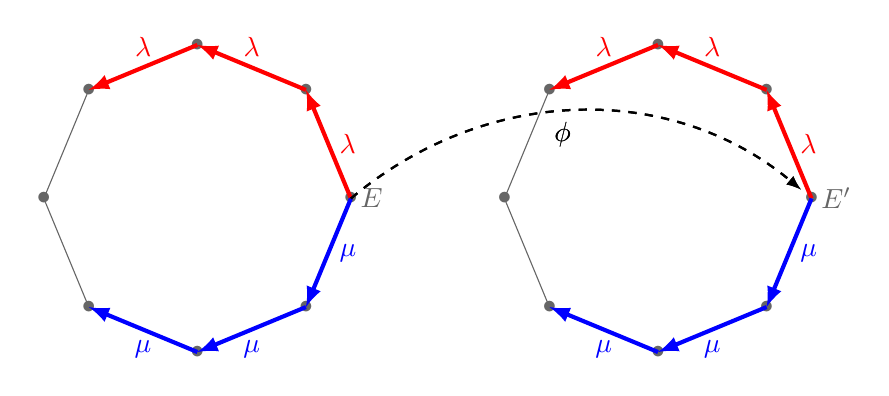
\begin{tikzpicture}[scale=0.39]
        \foreach \s/\e in {0/E,15cm/E'} {
          \begin{scope}[xshift=\s,black!60]
            \coordinate (A) at (0:5);
            \coordinate (B) at (45:5);
            \coordinate (C) at (90:5);
            \coordinate (D) at (135:5);
            \coordinate (E) at (180:5);
            \coordinate (F) at (225:5);
            \coordinate (G) at (270:5);
            \coordinate (H) at (315:5);

            \draw (A) node{$\bullet$};
            \draw (A) node[right]{$\e$};
            \draw (B) node{$\bullet$};
            \draw (C) node{$\bullet$};
            \draw (D) node{$\bullet$};
            \draw (E) node{$\bullet$};
            \draw (F) node{$\bullet$};
            \draw (G) node{$\bullet$};
            \draw (H) node{$\bullet$};

            \draw (A)--(B)--(C)--(D)--(E)--(F)--(G)--(H)--(A);		
            \begin{scope}[-latex]
              \draw[line width=1.5pt,red] (A)--(B) node[midway,right]{$\color{red} \lambda$};
              \draw[line width=1.5pt,blue] (A)--(H) node[midway,right]{$\color{blue} \mu$};
              \uncover<2->{
                \draw[line width=1.5pt,red] (B)--(C) node[midway,above]{$\color{red} \lambda$};
                \draw[line width=1.5pt,blue] (H)--(G) node[midway,below]{$\color{blue} \mu$};
              }
              \uncover<3->{
                \draw[line width=1.5pt,red] (C)--(D) node[midway,above]{$\color{red} \lambda$};
                \draw[line width=1.5pt,blue] (G)--(F) node[midway,below]{$\color{blue} \mu$};
              }
            \end{scope}
          \end{scope}

          \draw[dashed,thick,-latex,shorten >=5pt] (0:5) to[bend left=40] node[below left] {$\phi$} (0:20);
        }
      \end{tikzpicture}	
    \end{center}
  \end{figure}
\vspace{-4.5mm}
  \begin{uncoverenv}<3->
    \begin{itemize}
    \item On appelle $\red{E[\ell^k]_\lambda}\oplus\blu{E[\ell^k]_\mu}$ une
     décomposition \emph{horizontale};
    \item La littérature SEA appelle cela un \emph{cycle d'isogénies} [Couveignes,~Morain '94].%!!!!!!!!!!!!!!!!!!!!
    \end{itemize}
  \end{uncoverenv}

\end{frame}

%%%%%%%%%%%%%%%%%%%%%%%%%%%%%%%%%%%%%%%%%%%%%%%%%%%%%%%%%%%%

\begin{frame}

\bluebox{Un algorithme de Couveignes $\ell$-adique (cas Elkies $h=0$)}{
\begin{algorithmic}[1]
\REQUIRE $E, E',r$ tels que $E$ et $E'$ soient deux courbes $r$-isogènes sur $\mathbb{F}_{q}$ 
\ENSURE $\phi: E \rightarrow E'$ de degré $r$
\end{algorithmic}}

\bluebox{}{\textbf{Fait:} $\phi$ fait correspondre 
$\color{red}{E[\ell^k]_{{\lambda}}} \color{black}{\rightarrow} \color{red}{E'[\ell^k]_{{\lambda}}}$  
et 
$\color{blue}{E[\ell^k]_{{\mu}}} \color{black}{\rightarrow} \color{blue}{E'[\ell^k]_{{\mu}}}$.
 }

\begin{enumerate}
\item Choix du plus petit entier $k$ tel que $\ell^{2k}>4r$.
\medskip
\item Calcul de $\langle \red P , \blu Q \rangle = \color{red}{E[\ell^k]_{{\lambda}}} \color{black} \oplus \color{blue}{E[\ell^k]_{{\mu}}} $\\
 et $\langle \color{red} P' \color{black}, \color{blue} Q'\color{black} \rangle = \color{red}{E'[\ell^k]_{{\lambda}}} \color{black} \oplus \color{blue}{E'[\ell^k]_{{\mu}}} $ \hfill\only<2>{$\color{blue!50!gray}{\tilde{O}(r \ell^{O(1)})}$}
%\item Deduce $\to$ $\langle{\color{red}P},{\color{blue}Q}\rangle=E[\ell^k]$ and $\langle{\color{red}P'},{\color{blue}Q'}\rangle=E'[\ell^k]$;
\medskip
\item Pour toute matrice \textbf{diagonale inversible}
  $\left ( \begin{smallmatrix}a & 0\\ 0 & b
\end{smallmatrix}\right ) \in (\mathbb{Z}/\ell^k \mathbb{Z})^{2 \times 2}$:
\hfill\uncover<2>{$\color{blue!50!gray}{O(r)}$}
    \begin{enumerate}
  \item Calcul du polynôme d'interpolation 
    $L$  qui envoie\\
    $\color{red}P\mapsto [a]P'$ et $\color{blue}Q\mapsto [b]Q'$;
\hfill\uncover<2>{$\color{blue!50!gray}{\tilde{O}(r \ell^{O(1)})}$}
	\item Calcul d'une fraction rationnelle $F=L\bmod{T}$ de degrés \\
	$(r, r-1)$ et test de celle-ci.
\hfill\uncover<2>{$\color{blue!50!gray}{\tilde{O}(r)}$}
  \end{enumerate}
\end{enumerate}
\end{frame}

%%%%%%%%%%%%%%%%%%%%%%%%%%%%%%%%%%%%%%%%%%%%%%%%%%%%%%%%%%%%
%%%%%%%%%%%%%%%%%%%%%%%%%%%%%%%%%%%%%%%%%%%%%%%%%%%%%%%%%%%%
%\section{An $\ell$-adic Couveignes algorithm}


%%%%%%%%%%%%%%%%%%%%%%%%%%%%%%%%%%%%%%%%%%%%%%%%%%%%%%%%%%%%
\begin{frame}

\bluebox{Premier de Elkies}{Nous appelons $\ell$ un \emph{premier de Elkies} si le polynôme caractéristique de $\pi$ se factorise sur $\mathbb{Z}_{\ell}$ comme suit:
\[
\pi^2 - t_{\pi}\pi + q = (\pi - \red \lambda) (\pi - \blu \mu), \quad \textsf{avec } \red \lambda \neq \blu \mu,
\]
où $h=v_{\ell}(\red \lambda - \blu \mu)$ peut être $\geqslant 1$.
}
Comme pour tout $P \in  E[\ell^h]$ nous avons:
\[
\pi(P)= [\red \lambda ] P = [\blu \mu ] P
\]
nous ne pouvons directement distinguer les noyaux des isogénies de direction 
$\red \lambda$ de celles de direction $\blu \mu$.

\medskip
Ainsi dans l'algorithme de Couveignes  nous devons travailler avec $E[\ell^{k}]$ tel que $k \geqslant h+1$ afin de pouvoir déterminer $P \in \red{ E[\ell^{h+1}]_{ \lambda}}$ tel que: 
%Thus we have to work with $E[\ell^{h+1}]$ to get $P \in \red{ E[\ell^{h+1}]_{ \lambda}}$ such that:
\[
\pi(P)= [\red \lambda ] P \neq [\blu \mu ] P
\]
Nous supposons désormais que $k \geqslant h+1$.

\end{frame}


%
%\begin{frame}
%%Diapo sur le Frobenius....
%%We want to study the action of the Frobenius on the $\ell$ torsion:
%The Frobenius endomorphism acts on $E[\ell^k]$ as a $2\times2$ invertible matrix:
%\[
%\pi|E[\ell^k]:
%\begin{pmatrix}
%a & b \\
%c & d 
%\end{pmatrix} \bmod{\ell^k}
%\]
%%%%%%%%%%%%%%%%%%%%%%%%%%%%%%%%%%%%%%%%%%%%%%%%%%%%%%%%%%%%


\begin{frame}

\begin{prop}[De Feo, H., Pl\^ut, Schost, '16]\label{prop:matrice-Frobenius}
%Let $E$ be a curve on a crater of an $\ell$-isogeny volcano.
%Then there exists a unique $a \in \{ 0,\ell, \dots, \ell^{h-1}  \}$
%such that $\pi|T_\ell(E)$~is conjugate, over~$\mathbb{Z}_\ell$,
%to the matrix $\left ( \begin{smallmatrix}\lambda & a\\ 0 & \mu
%\end{smallmatrix}\right )$.
% where $a ∈ ℤ$, $0 ≤ a ≤ ℓ^{h} - 1$,
Dans le cas Elkies l'action de l'endomorphisme de Frobenius $\pi$ sur 
$E[\ell^{h+1}]$~est conjuguée, sur~$\mathbb{Z}_{\ell}$, à l'unique matrice
 \[\left ( \begin{matrix}{\color{red}\lambda} & a\\ 0 &
{\color{blue}\mu} \end{matrix}\right ), \]  avec $a \in \{ 1,\ell, \dots,
\ell^{h-1}, 0  \}$, et $a = 0$ ssi~$E$ se situe sur le cratère.

%Moreover $a = 0$ if~$E$ lies on the crater.
%and else $h - v_{\ell}(a)$~is the depth of~$E$ in the volcano.
\end{prop}

\begin{figure}
\begin{center}

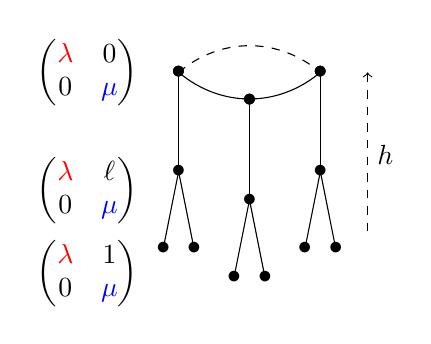
\begin{tikzpicture}[scale=0.30]
\coordinate (A) at (0,1.5);
\coordinate (AB) at (1,1.5);
\coordinate (AZ) at (-1.5,1.5);	
\coordinate (B) at (0,5);
\coordinate (BB) at (1,5);
\coordinate (BZ) at (-1.5,5.2);
\coordinate (BZ2) at (-1.5,4.8);
\coordinate (C) at (0,10);
\coordinate (CB) at (1,10);
\coordinate (CZ) at (-1.5,10);
\draw (A) node[left]{$\left( \begin{matrix}
\color{red}{\lambda} & 1 \\
0 & \color{blue}{\mu}
\end{matrix} \right) \color{black} $}; %node{$\bullet$};
\draw (B) node[left]{$ \left( \begin{matrix}
\color{red}{\lambda} & \ell \\
0 & \color{blue}{\mu}
\end{matrix} \right) \color{black} $}; %node{$\bullet$};
\draw (C) node[left]{$ \left( \begin{matrix}
\color{red}{\lambda} & 0 \\
0 & \color{blue}{\mu}
\end{matrix} \right) \color{black} $}; %node{$\bullet$};
%\draw (A)--(B);
%\draw (B)--(C);
%\draw (CZ)--(BZ)[dashed]  node[midway,left] {$\ell$};
%\draw (BZ2)--(AZ)[dashed]  node[midway,left] {$\ell$};
\begin{scope}[yshift=10cm]
	\begin{scope}[xshift=4.3cm]
		\node (A) at (-3,0) {$  \bullet $};
		\node (B) at (3,0) {$   \bullet$};
		\node (C) at (270:1.2) {$ \bullet \color{black}$};
		\node (D) at (90:1.5) {};
		%\draw[-] (A.center) to[bend right=25] (C.center);
		\draw[-,dashed] (A.center) to[bend left=40] (B.center);
		%\draw[-] (B.center) to[bend left=25] (C.center);
		%\draw[-,dashed] (B.center) to[bend right] (D.center);
		\draw[-] (A.center) to[bend right=40] (B.center);
		\draw (A) node{$  \bullet $};
		\draw (B) node{$  \bullet $};
		\draw (C) node{$  \bullet $};
		%\draw[line width=2.5pt,red,->] (A.center) to[bend right=20] (C.center);
			\begin{scope}[xshift=-3cm]
			\coordinate (A) at (0,0);
			\coordinate (C) at (270:4.2);
			\coordinate (CA) at (265:7.5);
			\coordinate (CB) at (275:7.5);
			\draw (C)--(CA);
			\draw (C)--(CB);
			\draw (A)--(C);
			\draw (CA) node{$ \bullet$};
			\draw (CB) node{$\bullet$};
			\draw (A) node{$  \bullet \color{black}$};
			\draw (C) node{$  \bullet \color{black}$};
			\end{scope}
			\begin{scope}[xshift=3cm]
			\coordinate (A) at (0,0);
			\coordinate (C) at (270:4.2);
			\coordinate (CA) at (265:7.5);
			\coordinate (CB) at (275:7.5);
			\draw (C)--(CA);
			\draw (C)--(CB);
			\draw (A)--(C);
			\draw (CA) node{$ \bullet$};
			\draw (CB) node{$\bullet$};
			\draw (A) node{$ \bullet$};
			\draw (C) node{$ \bullet$};
			\end{scope}
			\begin{scope}[yshift=-1.2cm]
			\coordinate (A) at (0,0);
			\coordinate (C) at (270:4.2);
			\coordinate (CA) at (265:7.5);
			\coordinate (CB) at (275:7.5);
			\draw (C)--(CA);
			\draw (C)--(CB);
			\draw (A)--(C);
			\draw (CA) node{$ \bullet$};
			\draw (CB) node{$ \bullet$};
			%\draw (A) node{$\bullet$};
			\draw (C) node{$ \bullet$};
			\draw (A) node{$ \bullet$};
			
			
			%(C) node[left]{$\mathcal{O}$} node{$\bullet$};			
			
			\end{scope}
			\coordinate (F) at (5,0);
			\coordinate (G) at (5,-7);
			\draw[dashed,<-] (F)--(G) node[midway,right]{$h$};
	\end{scope}
\end{scope}

%faire des fleches courbees avec les indices \ell et \ell^2

\end{tikzpicture}
\end{center}
\end{figure}
\end{frame}

%%%%%%%%%%%%%%%%%%%%%%%%%%%%%%%%%%%%%%%%%%%%%%%%%%%%%%%%%%%%


\begin{frame}
\frametitle{Marche sur le cratère}
%Does it work the same with general volcanoes of $\ell$-isogenies?
%\pause
Nous supposons que $E$ se situe sur le cratère (nous pouvons nous ramener facilement à ce cas).
 
%Let $P \in E[\ell^{h+1}]$ such that  $\pi(P)=\red \lambda(P)$
%We compute $\ell^k$-isogenies of kernel $\ker(\pi-\blu \mu)$.
\begin{columns}
\begin{column}{5cm}
\bluebox{Volcan de hauteur $h=0$}{
\begin{figure}[h]
	\begin{center}
	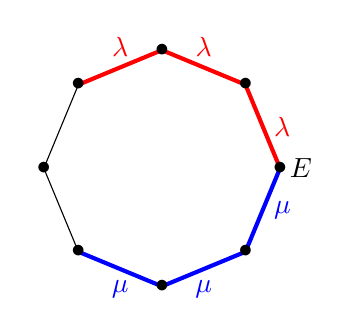
\begin{tikzpicture}[scale=0.3]
	\coordinate (A) at (0:5);
	\coordinate (B) at (45:5);
	\coordinate (C) at (90:5);
	\coordinate (D) at (135:5);
	\coordinate (E) at (180:5);
	\coordinate (F) at (225:5);
	\coordinate (G) at (270:5);
	\coordinate (H) at (315:5);
	\draw (A)--(B)--(C)--(D)--(E)--(F)--(G)--(H)--(A);		
	\draw[line width=1.5pt,red] (A)--(B) node[midway,right]{$\color{red} \lambda$};
	\draw[line width=1.5pt,blue] (A)--(H) node[midway,right]{$\color{blue} \mu$};
	\draw[line width=1.5pt,red] (B)--(C) node[midway,above]{$\color{red} \lambda$};
	\draw[line width=1.5pt,blue] (H)--(G) node[midway,below]{$\color{blue} \mu$};
	\draw[line width=1.5pt,red] (C)--(D) node[midway,above]{$\color{red} \lambda$};
	\draw[line width=1.5pt,blue] (G)--(F) node[midway,below]{$\color{blue} \mu$};
		
	\draw (A) node[right]{$E$};
	\draw (A) node{$\bullet$};
	\draw (B) node{$\bullet$};
	\draw (C) node{$\bullet$};
	\draw (D) node{$\bullet$};
	\draw (E) node{$\bullet$};
	\draw (F) node{$\bullet$};
	\draw (G) node{$\bullet$};
	\draw (H) node{$\bullet$};
	\end{tikzpicture}	
	\end{center}
\end{figure}
}
$\ker(\pi- \blu \mu\; | \; E[\ell^k])$ est un groupe cyclique de taille $\ell^k$.
\end{column}
\begin{column}{5.5cm}
\bluebox{Volcan de hauteur $h=2$}{\begin{center}
\tikzstyle{lambda1}=[lambda,draw=blue!60!green]
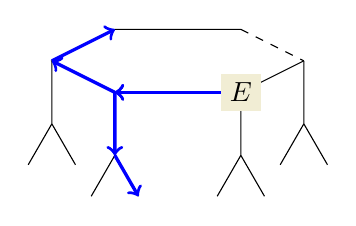
\begin{tikzpicture}[scale=0.40]
% \coordinate (A) at (0,-1.2);
% \coordinate (B) at (-3,0);
% \coordinate (C) at (-1.2,.7);
% \coordinate (D) at (1.2,.7);
% \coordinate (E) at (3,0);
\coordinate (A) at (2,-1);
\coordinate (B) at (-2,-1);
\coordinate (C) at (-4,0);
\coordinate (D) at (-2,1);
\coordinate (E) at (2,1);
\coordinate (F) at (4,0);
\draw (F)--(A)--(B)--(C)--(D)--(E); \draw[dashed] (E)--(F);

\coordinate[position=-90:.8 from A] (AA);
\coordinate[position=-60:.6 from AA] (AA0);
\coordinate[position=-120:.6 from AA] (AA1);
\draw (A)--(AA)--(AA0); \draw (AA)--(AA1);
\coordinate[position=-90:.8 from B] (BB);
\coordinate[position=-60:.6 from BB] (BB0);
\coordinate[position=-120:.6 from BB] (BB1);
\draw (B)--(BB)--(BB0); \draw (BB)--(BB1);
\coordinate[position=-90:.8 from C] (CC);
\coordinate[position=-60:.6 from CC] (CC0);
\coordinate[position=-120:.6 from CC] (CC1);
\draw (C)--(CC)--(CC0); \draw (CC)--(CC1);
\coordinate[position=-90:.8 from F] (FF);
\coordinate[position=-60:.6 from FF] (FF0);
\coordinate[position=-120:.6 from FF] (FF1);
\draw (F)--(FF)--(FF0); \draw (FF)--(FF1);
\draw<2>[lambda] (A)--(B); \draw<2>[lambda] (B)--(BB);
\draw<2>[lambda] (BB)--(BB0);
\draw<3>[lambda] (A)--(B); \draw<3>[lambda] (B)--(C);
\draw<3>[lambda] (C)--(D);
\node[fill=pacificcream] at (A) {$E$};
\end{tikzpicture}
\end{center}
}
\textbf{Problème:} si $h \geqslant 1$
alors $\ker(\pi- \blu \mu  \;| \; E[\ell^k])
\simeq (\mathbb Z/\ell^k) \!\times\! (\mathbb Z/\ell^h)$ n'est pas cyclique,
et contient $\ell^h$ sous-groupes cycliques d'ordre $\ell^k$.

\end{column}
\end{columns}

\end{frame}


%%%%%%%%%%%%%%%%%%%%%%%%%%%%%%%%%%%%%%%%%%%%%%%%%%%%%%%%%%%%

%\begin{frame}
%Our aim is to compute an horizontal decomposition: $E[\ell^k]_{\lambda} \oplus E[\ell^k]_{\mu}$ of $E[\ell^k]$ (aka isogeny cycle in the SEA litterature).

%We will proceed step by step since with diagonalisation of $\ker (\pi -\lambda), \ker (\pi -\mu)  \bmod \ell^{h+1}$ we get an horizontal decomposition $E[\ell^k]_{\lambda} \oplus E[\ell^k]_{\mu}$.


%\end{frame}

%%%%%%%%%%%%%%%%%%%%%%%%%%%%%%%%%%%%%%%%%%%%%%%%%%%%%%%%%%%%


\begin{frame}
\frametitle{Marche sur le cratère}

\bluebox{Fait}{
    Soit $\phi$ une $r$-isogénie avec $\ell \nmid r$, alors $\phi$ préserve les noyaux des $\ell^k$-isogénies horizontales de direction $\red \lambda, \blu \mu $.}
%\textbf{Goal:} compute the kernel of horizontal $\ell^k$-isogenies (codomain curves lying on the crater).
On procède étape par étape à l'aide de marche sur le cratère selon la direction $ \blu \mu$. %to compute the kernels of the horizontal $\ell^3$-isogeny of direction $\blu \mu $.
\vspace{-5mm}
\begin{center}
\begin{tikzpicture}[scale=0.37]
\begin{scope}[yshift=10cm]
	\begin{scope}[xshift=4.3cm]
		\node (A) at (-3,0) {$\bullet$};
		\node (B) at (3,0) {$\bullet$};
		\node (C) at (270:1.2) {$\bullet$};
		\node (D) at (125:1.2) {$E_2$};
		%\draw[-] (A.center) to[bend right=25] (C.center);
		\draw[-] (D.center) to[bend right=20] (A.center);
		\only<1-2>{		
		\draw[-] (D.center) to[bend left=18] (B.center);
		}
		\only<3->{
		\draw[line width=1.5pt,blue,->] (D.center) to[bend left=20] (B.center);
		
		\node (F) at (1.25,1.30) {$\color{blue} \mu$};
		%\node (F2) at (1.25,0.50) {$\color{blue} \psi_2$};		
		}
		\only<5->{
		\draw[line width=1.5pt,blue,->] (D.center) to[bend right=20] (A.center);		
		}
		\only<5->{		
		\node (F2) at (-2.25,1) {$\color{blue} \mu$};
		}
%		\only<4->{
%		\draw[line width=1.5pt,red,->] (D.center) to[bend left=20] (B.center);
%		\draw[-] (D.center) to[bend right=20] (A.center);
%		\node (F) at (1.25,1.30) {$\color{red} \lambda$};		
%		}
		%\draw[-] (B.center) to[bend left=25] (C.center);
		%\draw[-,dashed] (B.center) to[bend right] (D.center);
		\only<1->{
		\draw[line width=1.5pt,blue,->] (C.center) to[bend right=20] (B.center); 
		\node (F) at (1.5,-0.5) {$\color{blue} \mu$};	
		%\node (F2) at (1.5,-1.5) {$\color{blue} \psi$};	
		}
%		\only<2->{
%		\draw[line width=1.5pt,red,<-] (C.center) to[bend right=20] (B.center); 
%		\node (F) at (1.5,-0.5) {$\color{red} \lambda$};		
%		}
		
			\begin{scope}[xshift=-3cm]
			\coordinate (A) at (0,0);
			\coordinate (C) at (270:4.2);
			\coordinate (CA) at (265:7.5);
			\coordinate (CB) at (275:7.5);
			\draw (C)--(CA);
			\only<1>{
			\draw (C)--(CB);}
			\only<2->{
			\draw (C)--(CB);}
			\only<1-3>{			
			\draw (A)--(C);}
			\only<4->{
			\draw (A)--(C);}
			\only<5>{
			\draw [line width=1.5pt,blue] (C)--(A);
			\draw [line width=1.5pt,blue] (C)--(CA);
			}
			%just to have a 6th slide
			\only<6>{
			\draw (C)--(A);
			\draw (C)--(CA);
			}
%			\draw (A) node[fill=white]{$30$};
%			\draw (C) node[fill=white]{$98$};
%			\draw (CA) node[fill=white]{$22$};
%			\draw (CB) node[fill=white]{$74$};
			\draw (A) node[fill=white]{$E_3$};
			\draw (C) node[fill=white]{$\bullet$};
			\draw (CA) node[fill=white]{$\bullet$};
			\draw (CB) node[fill=white]{$\bullet$};
			\end{scope}
			\begin{scope}[xshift=3cm]
			\coordinate (A) at (0,0);
			\coordinate (C) at (270:4.2);
			\coordinate (CA) at (265:7.5);
			\coordinate (CB) at (275:7.5);
			\draw (C)--(CA);
			\draw (C)--(CB);
			\draw (A)--(C);
			\only<1>{
			\draw [line width=1.5pt,blue] (C)--(CB);
			\draw [line width=1.5pt,blue] (A)--(C);
			}
%			\draw (A) node[fill=white]{$65$};
%			\draw (C) node[fill=white]{$60$};
%			\draw (CA) node[fill=white]{$39$};
%			\draw (CB) node[fill=white]{$62$};
			\draw (A) node[fill=white]{$E_1$};
			\only<2-3>{\draw (A) node[fill=yellow!50!white,shape=circle]{$E_1$};}
			\draw (C) node[fill=white]{$\bullet$};
			\draw (CA) node[fill=white]{$\bullet$};
			\draw (CB) node[fill=white]{$\bullet$};
			\end{scope}
			\begin{scope}[yshift=-1.2cm]
			\coordinate (A) at (0,0);
			\coordinate (C) at (270:4.2);
			\coordinate (CA) at (265:7.5);
			\coordinate (CB) at (275:7.5);
			\draw (C)--(CA);
			\draw (C)--(CB);
			\draw (A)--(C);
			\draw (A) node[fill=white]{$E$};
			\only<1>{\draw (A) node[fill=yellow!50!white,shape=circle]{$E$};}
			\draw (C) node[fill=white]{$\bullet$};
			\draw (CA) node[fill=white]{$\bullet$};
			\draw (CB) node[fill=white]{$\bullet$};
%			\draw (CA) node[fill=white]{$45$};
%			\draw (CB) node[fill=white]{$68$};
			\end{scope}
			\begin{scope}[shift={(D)}]
			\coordinate (A) at (0,0);
			\coordinate (C) at (270:4.2);
			\coordinate (CA) at (265:7.5);
			\coordinate (CB) at (275:7.5);
			\draw [dashed] (C)--(CA);
			\draw [dashed] (C)--(CB);
			\draw [dashed] (A)--(C);
			\draw (C) node[color=black!90]{$\bullet$};
			\draw (CA) node[color=black!90]{$\bullet$};
			\draw (CB) node[color=black!90]{$\bullet$};
			\only<3>{
			\draw [line width=1.5pt,blue] (C)--(A);
			\draw [line width=1.5pt,blue] (C)--(CA);
			}
			\only<1-3,5->{\draw (A) node[fill=white]{$E_2$};}			
			\only<4>{\draw (A) node[fill=yellow!50!white,shape=circle]{$E_2$};}
			\end{scope}
	\coordinate (A) at (-3,0);
	\coordinate (C) at (270:1.2);
	\only<1->{
	\draw (A.center) to[bend right=20] (C.center);
	}
	\draw (A) node[fill=white]{$E_3$};
	\only<1>{
	\draw (C) node[fill=yellow!50!white,shape=circle]{$E$};
	}	
	\only<2->{
	\draw (C) node[fill=white]{$E$};
	}
	\end{scope}
\end{scope}

\end{tikzpicture}
\end{center}
\vspace{-4mm}
D'autres algorithmes pour déterminer des isogénies horizontales ont déjà été proposés: [Fouquet, Morain, '02], [Ionica,Joux, '10].
\end{frame}

%%%%%%%%%%%%%%%%%%%%%%%%%%%%%%%%%%%%%%%%%%%%%%%%%%%%%%%%%

\begin{frame}

\bluebox{Un algorithme de Couveignes $\ell$-adique ($\ell$ un premier de Elkies)}{
\begin{algorithmic}[1]
\REQUIRE $E, E',r$ tels que $E$ et $E'$ soient deux courbes $r$-isogènes sur $\mathbb{F}_{q}$ 
\ENSURE $\phi: E \rightarrow E'$ de de degré $r$
\end{algorithmic}}

\bluebox{}{\textbf{Fait:} $\phi$ fait correspondre 
$\color{red}{E[\ell^k]_{{\lambda}}} \color{black}{\rightarrow} \color{red}{E'[\ell^k]_{{\lambda}}}$  
et
$\color{blue}{E[\ell^k]_{{\mu}}} \color{black}{\rightarrow} \color{blue}{E'[\ell^k]_{{\mu}}}$.
 }

\begin{enumerate}
\item Calcul du plus petit entier $k$ tel que $\ell^{2k}>4r$, avec $h<k$.
\medskip
\item Calcul de $\langle \red P , \blu Q \rangle = \color{red}{E[\ell^k]_{{\lambda}}} \color{black} \oplus \color{blue}{E[\ell^k]_{{\mu}}} $\\
 et $\langle \color{red} P' \color{black}, \color{blue} Q'\color{black} \rangle = \color{red}{E'[\ell^k]_{{\lambda}}} \color{black} \oplus \color{blue}{E'[\ell^k]_{{\mu}}} $ générateurs de $\ell^k$-isogénies horizontales de directions $\color{red} \lambda \color{black}, \color{blue} \mu$. \hfill\uncover<2>{$\color{blue!50!gray}{\tilde{O}(r \ell^{O(1)})}$}  
%\item Deduce $\to$ $\langle{\color{red}P},{\color{blue}Q}\rangle=E[\ell^k]$ and $\langle{\color{red}P'},{\color{blue}Q'}\rangle=E'[\ell^k]$; Rajouter le coût de cela...
\medskip
\item Pour toute matrice \textbf{diagonale inversible}
  $\left ( \begin{smallmatrix}a & 0\\ 0 & b
\end{smallmatrix}\right ) \in (\mathbb{Z}/\ell^k \mathbb{Z})^{2 \times 2}$:
\hfill\uncover<2>{$\color{blue!50!gray}{O(r)}$}
  \begin{enumerate}

%  \item Calcul du polynôme d'interpolation 
%    $L$ qui envoie\\
%    $\color{red}P\mapsto [a]P'$ et $\color{blue}Q\mapsto [b]Q'$;
%\hfill\only<2>{$\color{blue!50!gray}{\tilde{O}(r \ell^{O(1)})}$}
%	\item Utilisation d'un algorithme de reconstruction rationnelle afin de 
%	calculer une fraction rationnelle $F$ de degrés~$(r, r-1)$;
%\hfill\only<2>{$\color{blue!50!gray}{\tilde{O}(r)}$}
%  \item Si $F$ définit une isogénie de degré $r$, on la retourne et on termine
%   l'algorithme.
   
   \item Calcul et test d'un candidat à l'aide d'un polynôme d'interpolation \\
   $L$ qui envoie $\color{red}P\mapsto [a]P'$ et $\color{blue}Q\mapsto [b]Q'$; \hfill\uncover<2>{$\color{blue!50!gray}{\tilde{O}(r \ell^{O(1)})}$}
  \end{enumerate}
\end{enumerate}
\end{frame}

%%%%%%%%%%%%%%%%%%%%%%%%%%%%%%%%%%%%%%%%%%%%%%%%%%%%%%%%%%%%

\begin{frame}
\frametitle{Limitations du cas Elkies}
 \bluebox{Trouver un premier $\ell$ de Elkies}{
  \begin{itemize}
  \item La complexité de l'algorithme dépend polynomialement du paramètre $\ell$.
  \item Heuristiquement la moitié des paramètres $\ell$ sont supposés être des premiers de Elkies.
  \item En théorie nous pouvons seulement prouver qu'un tel $\ell \leqslant 
  O(\log(q))$ pour presque tous les $q$ et courbes $E,E'$ (voir 
[Shparlinski,~Sutherland~'14]).\\
 $\Rightarrow$ Algorithme quasi-quadratique de Couveignes $\ell$-adique.
\end{itemize}
  }
\end{frame}
%%%%%%%%%%%%%%%%%%%%%%%%%%%%%%%%%%%%%%%%%%%%%%%%%%%%%%%%%%%% 
%\section{Algorithme de Couveignes $\ell$-adique}

\begin{frame}
%\section{Atkin Case}
\frametitle{Cas Atkin}
\bluebox{Premier de Atkin}{Un nombre premier $\ell$ est dit un \emph{premier de Atkin} si le polynôme caractéristique de $\pi$: 
\[
\pi^2 - t\pi + q 
\]
est irréductible sur $\mathbb{Z}_{\ell}$}
%Thus we are not able to distinguish two different eigenspaces, 
Ainsi on ne peut se servir d'isogénies horizontales comme ce fut le cas avec des \emph{premiers de Elkies}.  
\begin{figure}
\begin{center}
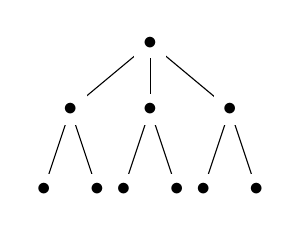
\begin{tikzpicture}[scale=0.225]
\begin{scope}[yshift=10.5cm,xshift=6.3cm,scale=0.75]
		\coordinate (D) at (0,0);
		\coordinate (E) at (-6,-5);
		\coordinate (F) at (6,-5);
		\coordinate (G) at (-4,-11);
		\coordinate (H) at (-8,-11);
		\coordinate (I) at (4,-11);
		\coordinate (J) at (8,-11);
		\coordinate (K) at (0,-5);
		\coordinate (L) at (-2,-11);
		\coordinate (M) at (2,-11);
		\draw (D) -- (E);
		\draw (D) -- (F);
		\draw (D) -- (K);
		\draw (K) -- (L);
		\draw (K) -- (M);
		\draw (E) -- (H);
		\draw (E) -- (G);
		\draw (F) -- (I);
		\draw (F) -- (J);
		%\coordinate (G) at (E)++(225:3);
		\draw (D) node[fill=white]{$\bullet$};
		\draw (J) node[fill=white]{$\bullet$};
		\draw (E) node[fill=white]{$\bullet$};
		\draw (F) node[fill=white]{$\bullet$};
		\draw (G) node[fill=white]{$\bullet$};
		\draw (H) node[fill=white]{$\bullet$};
		\draw (I) node[fill=white]{$\bullet$};
		\draw (K) node[fill=white]{$\bullet$};
		\draw (L) node[fill=white]{$\bullet$};
		\draw (M) node[fill=white]{$\bullet$};
\end{scope}
\end{tikzpicture}
\end{center}
\end{figure}
\end{frame}

%%%%%%%%%%%%%%%%%%%%%%%%%%%%%%%%%%%%%%%%%%%%%%%%%%%%%%%%%%%

\begin{frame}
\frametitle{Détermination du second vecteur de la base à l'aide du Frobenius}
\begin{nota}
La notation $M_{\pi}(P,Q)$ désigne l'action du Frobenius dans une base $\langle P,Q \rangle = E[\ell^k]$
\end{nota}

\textbf{Exemple :}Pour deux points $P_0$ et $Q_0$ générateurs de $\ell^k$-isogénies horizontales 
\[
M_{\pi}(P_0,Q_0)= \left( \begin{smallmatrix} \color{red}{\lambda} & \color{black} 0 \\
0 & \color{blue} \mu \end{smallmatrix} \right)
\]

\begin{prop}
Soit $E$ située sur un volcan de hauteur $0$, $\ell$ un nombre premier de 
Atkin, $P,Q,R$ trois points de $E$  tels que $\langle P,Q \rangle = \langle P,R 
\rangle =E[\ell^k] $ alors $Q=R \Leftrightarrow M_{\pi}(P,Q)=M_{\pi}(P,R)$. 
\end{prop}
\end{frame}
%%%%%%%%%%%%%%%%%%%%%%%%%%%%%%%%%%%%%%%%%%%%%%%%%%%%%%%%%%%
\begin{frame}

\bluebox{Un algorithme de Couveignes $\ell$-adique (Cas Atkin $h = 0$)}{
\begin{algorithmic}[1]
\REQUIRE $E, E',r$ tels que $E$ et $E'$ soient deux courbes $r$-isogènes sur $\mathbb{F}_{q}$ 
\ENSURE $\phi: E \rightarrow E'$ de degré $r$
\end{algorithmic}}

\bluebox{}{\textbf{Fait:} $M_{\pi}(P,R)=M_{\pi}(P,Q)$ ssi $R=Q$ 
avec $\langle P,R \rangle = \langle P,Q \rangle = E[\ell^{k}]$.}

\begin{enumerate}
\item Choix du plus petit entier $k$ tel que $\ell^{2k}>4r$.
\medskip
\item Calcul de $\langle P , Q \rangle = E[\ell^k]$ et $\langle P' , Q' \rangle = E'[\ell^k]$; \hfill\only<2>{$\color{blue!50!gray}\tilde{O}(r \ell^{O(1)})$}
%\item Deduce $\to$ $\langle{\color{red}P},{\color{blue}Q}\rangle=E[\ell^k]$ and $\langle{\color{red}P'},{\color{blue}Q'}\rangle=E'[\ell^k]$;
\medskip
\item Calcul de la matrice $M_{\pi}(P,Q)$; \hfill\uncover<2>{$\color{blue!50!gray}{\tilde{O}(\sqrt{r}\ell^{O(1)})}$}
\medskip
\item Pour tout point $S'$ d'ordre $\ell^k$ de $E'$: \hfill\uncover<2>{$\color{blue!50!gray}{O(r)}$}
\begin{enumerate}
\medskip
  \item Calcul de $R'$ tel que $\pi(S',R')=\pi(P,Q)$ \hfill\only<2>{$\color{blue!50!gray}{\tilde{O}(\sqrt{r} \ell^{O(1)})}$}
  \medskip

%  \item Calcul du polynôme d'interpolation 
%    $L$ qui envoie\\
%    $P\mapsto S'$ et $Q\mapsto R'$;
\item Calcul et test d'un candidat à l'aide d'un polynôme d'interpolation \\
   $L$ qui envoie $P\mapsto S'$ et $Q\mapsto R'$; \hfill\only<2>{$\color{blue!50!gray}{\tilde{O}(r \ell^{O(1)})}$}
   \end{enumerate}
\end{enumerate}
\end{frame}


%%%%%%%%%%%%%%%%%%%%%%%%%%%%%%%%%%%%%%%%%%%%%%%%%%%%%%%

\begin{frame}

\bluebox{Un algorithme de Couveignes $\ell$-adique (Cas Atkin $h \neq 0$)}{
\begin{algorithmic}[1]
\REQUIRE $E, E',r$ tels que $E$ et $E'$ soient deux courbes $r$-isogènes sur $\mathbb{F}_{q}$ 
\ENSURE $\phi: E \rightarrow E'$ de degré $r$
\end{algorithmic}}
\only<1>{
\bluebox{}{\textbf{Fait:} $\pi(P,R)=\pi(P,Q)$ ssi $\color{red}[\ell^h]\color{black}R=\color{red}[\ell^h]\color{black}Q$ \\
avec $\langle P,R \rangle = \langle P,Q \rangle = E[\ell^{h+i}]$ avec $i>0$.}
}
\only<2>{
\bluebox{}{\textbf{Fait:} $\pi(P,R)=\pi(P,Q)$ ssi $[\ell^h]R=[\ell^h]Q$ \\
avec $\langle P,R \rangle = \langle P,Q \rangle = E[\ell^{h+i}]$ avec $i>0$.}
}
\begin{enumerate}
\item Choix du plus petit entier $k$ tel que $\ell^{2k}>4r$.
\medskip
\item Calcul de $\langle P , Q \rangle = E[\ell^k]$ et $\langle P' , Q' \rangle = E'[\ell^k]$; \hfill{$\color{blue!50!gray} \tilde{O}(r \ell^{O(1)})$}
%\item Deduce $\to$ $\langle{\color{red}P},{\color{blue}Q}\rangle=E[\ell^k]$ and $\langle{\color{red}P'},{\color{blue}Q'}\rangle=E'[\ell^k]$;
\medskip
\item Calcul de la matrice $\pi(P,Q)$; \hfill {$\color{blue!50!gray} \tilde{O}(\sqrt{r} \ell^{O(1))})$}
\medskip
\item Pour tout point $S'$ d'ordre $\ell^k$ de $E'$: \hfill {$\color{blue!50!gray}{O(r)}$}
\begin{enumerate}
\medskip
  \item Calcul de $R'$ tel que $\pi(S',R')=\pi(P,Q)$ \hfill {$\color{blue!50!gray}{\tilde{O}(\sqrt{r} \ell^{O(1)})}$}
  \medskip
  \only<1>{
  \item $\color{red}{\text{Pour tout point } U' \in E' \text{ tel que } [\ell^h]R'=[\ell^h]U'}$}
  \only<2>{
  \item Pour tout point $U' \in E'$ tel que $[\ell^h]R'=[\ell^h]U'$ \hfill {$\color{blue!50!gray}{O(\ell^h)}$}}
  \begin{enumerate}

%  \item Calcul du polynôme d'interpolation 
%    $L$ qui envoie\\
%    $P\mapsto S'$ et $Q\mapsto U'$;
%\hfill {$\color{blue!50!gray}{\tilde{O}(r \ell^{O(1)})}$}
\item Calcul et test d'un candidat à l'aide d'un polynôme d'interpolation \\
   $L$ qui envoie $P\mapsto S'$ et $Q\mapsto U'$; \hfill $\color{blue!50!gray}{\tilde{O}(r \ell^{O(1)})}$
  \end{enumerate}
	
\end{enumerate}
\end{enumerate}
\end{frame}

%%%%%%%%%%%%%%%%%%%%%%%%%%%%%%%%%%%%%%%%%%%%%%%%%%%%%%%%%%%%%

\begin{frame}
\frametitle{Algorithme de Couveignes $\ell$-adique}

\begin{thm}
Soient $q$ une puissance d'un nombre premier, deux courbes elliptiques $E,E'$
définies sur $\mathbb{F}_q$, un entier $r$ tel que $E$ et $E'$ soient 
$r$-isogènes, alors la $r$-isogénie peut être calculée avec une complexité de
\[
\tilde{O}(r^2 \ell^{O(1)}) \text{ opérations sur }\mathbb{F}_q
\]
avec un paramètre $\ell$ borné par $O(\log(q))$.
\end{thm}

\end{frame}

%%%%%%%%%%%%%%%%%%%%%%%%%%%%%%%%%%%%%%%%%%%%%%%%%%%%%%%%%%%%
\section{Implantation}

\begin{frame}
\frametitle{Construction et définition d'une tour d'extension de corps finis}
\begin{columns}
\begin{column}{2cm}
\begin{center}
\begin{figure}
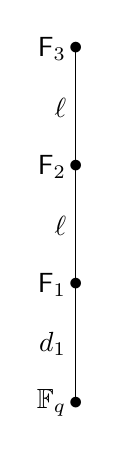
\begin{tikzpicture}[scale=0.3]
\coordinate (A) at (-2,0);	
\coordinate (B) at (-2,5);
\coordinate (C) at (-2,10);
\coordinate (D) at (-2,15);
\draw (A) node {$\bullet$} node[left] {$\mathbb{F}_q$};
\draw (B) node {$\bullet$} node[left] {$\mathsf{F}_1$};
\draw (C) node {$\bullet$} node[left] {$\mathsf{F}_2$};
\draw (D) node {$\bullet$} node[left] {$\mathsf{F}_3$};
\draw (C)--(D) node[midway,left]{$\ell$} ;
\draw (B)--(C) node[midway,left]{$\ell$} ;
\draw (A)--(B) node[midway,left]{$d_1$} ;
\end{tikzpicture}
\end{figure}
\end{center}
\end{column}
\begin{column}{8cm}

\begin{defi}[Tour \textit{$\ell$}-adique]
Pour $\ell \neq p$ la caractéristique de $\mathbb{F}_q$, une tour d'extensions 
$\ell$-adiques de $\mathbb{F}_q$ est une suite d'extensions: $\mathbb{F}_q, 
\mathsf{F}_{1}, \mathsf{F}_{2}, \mathsf{F}_{3}, \cdots$ telles que:
\begin{itemize}
\item{} [Cas Elkies] $\mathsf{F}_{1}$ est une extension de $\mathbb{F}_q$ de 
degré $d_1 \mid \ell-1$. De plus l'ordre multiplicatif de $q$ dans 
$\mathbb{Z}/\ell \mathbb{Z}$ divise $d_1$,
\item{} [Cas Atkin] $\mathsf{F}_{1}$ est une extension de $\mathbb{F}_q$ de 
degré au plus $ \ell^2-1$,
\item $\mathsf{F}_{i}$ pour $i \geqslant 2$ est une extension de 
$\mathsf{F}_{i-1}$ de degré $\ell$.
\end{itemize}

\end{defi}
\end{column}
\end{columns}
\end{frame}

%%%%%%%%%%%%%%%%%%%%%%%%%%%%%%%%%%%%%%%%%%%%%%%%%%%%%%%%%%%%%%%%%%%%%%%%

\begin{frame}

  \frametitle{Tour d'extensions de corps finis}

  \bluebox{Calcul dans une tour d'extension de corps finis}{
  \begin{itemize}
%	\item Les points de torsion ne sont pas en général définis dans $\mathbb{F}_q$.	
	\item Nous travaillons dans des extensions $\ell$-adiques de $\mathbb F_q$
        en généralisant les constructions de [De~Feo,~Doliskani, Schost '13], [Doliskani,~Schost '15] et où en particulier nous avons
		\begin{itemize}  
		 \item un calcul rapide des points d'ordre $\ell^k$,       
         \item un calcul rapide du Frobenius (adapté depuis [Doliskani-Schost'15]),
         \item un calcul rapide du polynôme d'interpolation (adaptant des 
         techniques de [Enge,Morain~'03] développées par [De Feo~'10])
         \end{itemize}
\end{itemize}
 	
  }

\end{frame}


%%%%%%%%%%%%%%%%%%%%%%%%%%%%%%%%%%%%%%%%%%%%%%%%%%%%%%%%%%%%

\begin{frame}
\frametitle{Expérimentations}
L'algorithme (cas Elkies) a été implanté sur SageMath v7.1 seulement pour $\ell=2$, le code ($2200$ lignes) est disponible sur GitHub: \url{https://github.com/Hugounenq-Cyril/Two_curves_on_a_volcano}
\begin{figure}[hbtp]
\centering
\only<2>{
\includegraphics[scale=0.8]{Images/graphe-101-149-269-C2.pdf}}
\only<1>{
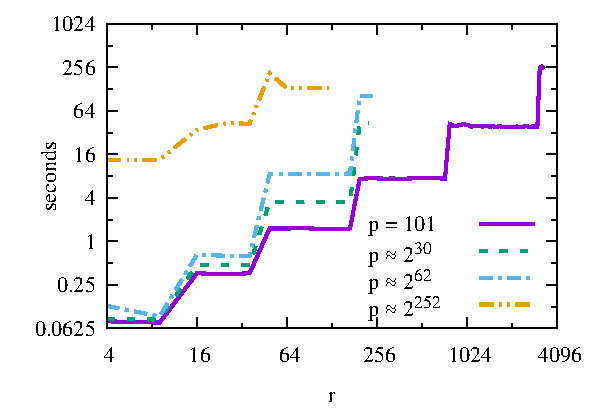
\includegraphics[scale=0.8]{Images/graphe-101-149-269.pdf}}
\end{figure}
\end{frame}


%%%%%%%%%%%%%%%%%%%%%%%%%%%%%%%%%%%%%%%%%%%%%%%%%%%%%%%%%%%% 

\begin{frame}
\frametitle{Conclusion}
\bluebox{Contribution}{
\begin{itemize}
\item De nouveaux outils pour se déplacer dans le volcan d'isogénies. 

\item Une variante de l'algorithme de Couveignes quasi-quadratique.

\end{itemize}
}
\bluebox{Travaux futurs}{
\begin{itemize}
\item Comparer notre implantation à d'autres algorithmes (en part. Lercier-Sirvent dans le contexte S.E.A.).
% \item Directly generalize to curves not on the crater.
\item Estimer le coût de calcul de l'anneau des endomorphismes en modifiant l'algorithme de Kohel'96  avec l'étude de l'action de l'endomorphisme de Frobenius et l'implanter.
\item Étudier l'utilité de notre technique dans d'autres contextes: comptage de points, polynômes de Hilbert, polynômes modulaires.
%Analyze our techniques to navigate the volcano in other
%  settings: point counting, Hilbert
%  class polynomials, modular polynomials.
\item Résoudre le problème de l'isogénie explicite avec une complexité de $\tilde{O}(r)$ opérations sur $\mathbb{F}_q$.
\end{itemize}}

%Code available on GitHub: \url{https://github.com/Hugounenq-Cyril/Two_curves_on_a_volcano}
\end{frame}

% \begin{frame} 

% \bibliography{Biblio}
% \end{frame}

\setbeamertemplate{headline}{\relax}
\setbeamertemplate{footline}{\relax}
\begin{frame}
\begin{center}
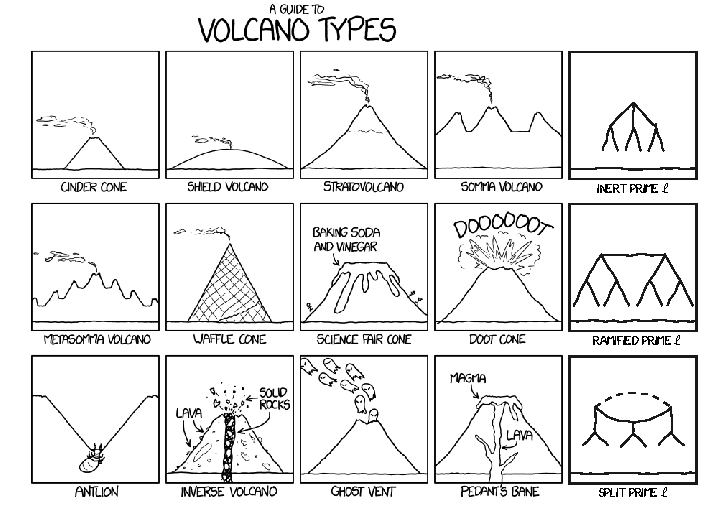
\includegraphics[width=.9\hsize]{Images/volcan}
\end{center}
\tiny Modified from  \href{http://xkcd.com/1714/}{xkcd.com/1714}
\end{frame}

%%%%%%%%%%%%%%%%%%%%%%%%%%%%%%%%%%%%%%%%%%%%%%%%%%%%%%%%%%%%
\backupbegin
\begin{frame}
\frametitle{Détails techniques: Amélioration de l'interpolation avec le Frobenius}
%$A$ the polynomial that interpolates the isogeny according to the mappings $\red P \rightarrow \color{red} u P' $, $\blu Q \rightarrow \color{blue}v Q'$  and $\color{red} P' \in  E'[\ell^k]_{\lambda}$, $\color{blue} Q' \in  E'[\ell^k]_{\mu} \color{black}$.

%$T$ the polynomial that interpolates the isogeny according to the mapping \[P \mapsto a P \quad Q \mapsto bQ \quad \textit{with } a,b \wedge \ell = 1.\]
Nous cherchons à calculer une $\mathbb{F}_q$ isogénie \textbf{rationnelle}, ainsi pour tout polynôme d'interpolation candidat $L$ nous avons pour $R \in E[\ell^k]$: 
\[\pi(L(x(R)))=L(x(\pi(R))),\]
et en particulier avec $\color{red} P \in  E[\ell^k]_{\lambda}$, $\color{blue} Q \in  E[\ell^k]_{\mu} \color{black}$:
\[\pi(L(x(\red P)))=L(x(\color{red} \lambda P \color{black}))) \quad \pi(L(x(\blu Q)))=L(x(\color{blue} \mu Q \color{black}))).\]
\pause
Comme suggéré par [Couveignes,96] on calcule $L$ séparément sur les points représentants des orbites sous l'action du Frobenius: 
\[
\{ {\boldmath \color{red} \textbf{P}} \unboldmath , \pi(\red P), \pi^2(\red P), \cdots \color{black} \}  
\]
\[
\{ {\boldmath \color{blue} \textbf{Q}} \unboldmath , \pi(\blu Q), \pi^2(\blu Q), \cdots \color{black} \}  
\]
\[
\cdots
\]
nous utilisons ensuite le Théorème des Restes Chinois pour obetnir $L$.

\end{frame}

%%%%%%%%%%%%%%%%%%%%%%%%%%%%%%%%%%%%%%%%%%%%%%%%%%%%%%%%%%%% 
%%%%%%%%%%%%%%%%%%%%%%%%%%%%%%%%%%%%%%%%%%%%%%%%%%%%%%%%%%%% 


\begin{frame}
\frametitle{Détails techniques: Amélioration de l'interpolation avec le Frobenius}
\begin{figure}[h]
\begin{center}

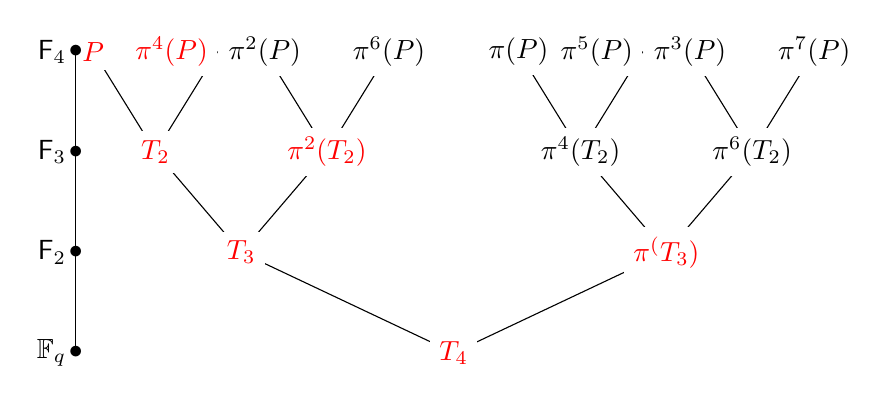
\begin{tikzpicture}[scale=0.3]
        \coordinate (A) at (0,0);
        \coordinate (AB) at (-9,4.25);
		\coordinate (AC) at (9,4.25);
		\draw (A)--(AB);
		\draw (A)--(AC);
		\draw (A) node[fill=white]{$\color{red}{T_4}$};
		

		\coordinate (ABA) at (-12.63,8.5);
		%\coordinate (ABA) at (-11.63,8.5);
		
		\draw (ABA)--(AB);
		
		\coordinate (ABAb) at (-15.26,12.75);
		%\coordinate (ABAb) at (-14.26,12.75);
		
		\draw (ABA)--(ABAb);
		\draw (ABAb) node[fill=white]{$\color{red}{P}$};
		
		\coordinate (ABAa) at (-10,12.75);
		%\coordinate (ABAa) at (-9,12.75);
		
		
		\draw (ABA)--(ABAa);
		\draw (ABA) node[fill=white]{$\color{red}{T_2}$};
		\draw (ABAa) node[fill=white][left]{$\color{red}{\pi^4(P)}$};%ancien \pi(T)
		
		\coordinate (ACA) at (-5.37,8.5);
		%\coordinate (ACA) at (-6.37,8.5);
		
		
		\draw (AB)--(ACA);
		\draw (AB) node[fill=white]{$\color{red}{T_3}$};
		\coordinate (ACAa) at (-8,12.75);
		%\coordinate (ACAa) at (-9,12.75);
		
		
		\draw (ACA)--(ACAa);
		\draw (ACAa) node[fill=white]{$\pi^2(P)$};%ancien \pi^2(T)
		
		\coordinate (ACAb) at (-2.74,12.75);
		%\coordinate (ACAb) at (-3.74,12.75);
		
		
		\draw (ACA)--(ACAb);
		\draw (ACAb) node[fill=white]{$\pi^6(P)$};%ancien \pi^3(T)
		\draw (ACA) node[fill=white]{$\color{red}{\pi^2(T_2)}$};% ancien \pi^2(T_2)
		
		\begin{scope}[xshift=18cm]
		\coordinate (ABA) at (-12.63,8.5);
		%\coordinate (ABA) at (-11.63,8.5);

		\draw (ABA)--(AC);
		
		\coordinate (ABAb) at (-15.26,12.75);
		%\coordinate (ABAb) at (-14.26,12.75);
		
		\draw (ABA)--(ABAb);
		\draw (ABAb) node[fill=white]{$\pi(P)$};%ancien \pi^4(T)
		
		\coordinate (ABAa) at (-10,12.75);
		%\coordinate (ABAa) at (-9,12.75);
		
		
		\draw (ABA)--(ABAa);
		\draw (ABAa) node[fill=white,left]{$\pi^5(P)$};%ancien \pi^5(T)
		\draw (ABA) node[fill=white]{$\pi^4(T_2)$};%ancien \pi^4(T_2)
		
		\coordinate (ACA) at (-5.37,8.5);
		%\coordinate (ACA) at (-6.37,8.5);
		
		
		\draw (AC)--(ACA);
		\draw (AC) node[fill=white]{$\color{red}{\pi^(T_3)}$};%ancien \pi^4(T_3)
		
		\coordinate (ACAa) at (-8,12.75);
		%\coordinate (ACAa) at (-9,12.75);
		
		
		\draw (ACA)--(ACAa);
		\draw (ACAa) node[fill=white]{$\pi^3(P)$};%ancien \pi^6(T)
		
		\coordinate (ACAb) at (-2.74,12.75);
		%\coordinate (ACAb) at (-3.74,12.75);
		
		
		\draw (ACA)--(ACAb);
		\draw (ACAb) node[fill=white]{$\pi^7(P)$};%ancien \pi^7(T)	
		\draw (ACA) node[fill=white]{$\pi^6(T_2)$};%ancien \pi^6(T_2)	
		\end{scope}
		
		\coordinate (A1) at (-16,0);
		\coordinate (A2) at (-16,4.25);
		\coordinate (A3) at (-16,8.5);
		\coordinate (A4) at (-16,12.75);
		\draw (A1)--(A2)--(A3)--(A4);
		\draw (A1) node{$\bullet$};
		\draw (A2) node{$\bullet$};
		\draw (A3) node{$\bullet$};
		\draw (A4) node{$\bullet$};
		\draw (A1) node[left]{$\mathbb{F}_q$};
		\draw (A2) node[left]{$\mathsf{F}_{2}$};
		\draw (A3) node[left]{$\mathsf{F}_{3}$};
		\draw (A4) node[left]{$\mathsf{F}_{4}$};
\end{tikzpicture}

\end{center}
\end{figure}
%Elements of the binary tree we need for the computation of the interpolation polynomial.
Éléments de l'arbre de produit binaire nécessaires au calcul du polynôme d'interpolation.
\end{frame}


%%%%%%%%%%%%%%%%%%%%%%%%%%%%%%%%%%%%%%%%%%%%%%%%%%%%%%%%%%%%%%%%%%%%%%

\begin{frame}
\frametitle{Points ascendants horizontaux}
\begin{figure}
\begin{center}
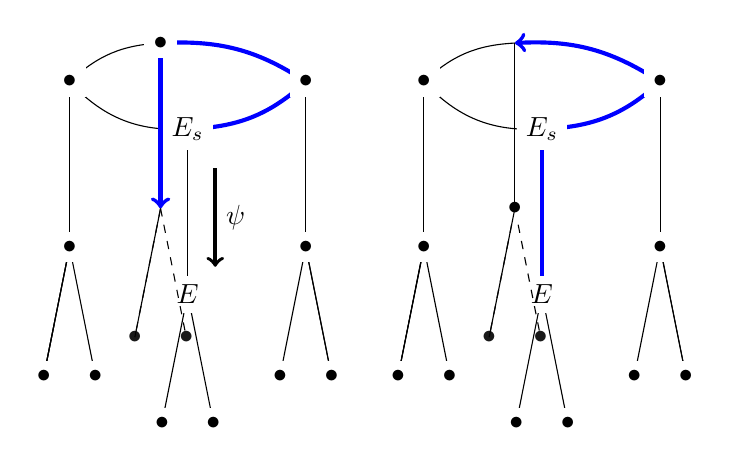
\begin{tikzpicture}[scale=0.50]
\begin{scope}%[yshift=10cm]
	\begin{scope}[xshift=4.3cm]
		%Cratere
		\node (A) at (-3,0) {$\bullet$};
		\node (B) at (3,0) {$\bullet$};
		\node (C) at (270:1.2) {$\bullet$};
		\node (D) at (125:1.2) {$\bullet$};
		\draw[-] (A.center) to[bend right=25] (C.center);
		\draw[-] (D.center) to[bend right=20] (A.center);	
		\draw[line width=1.5pt,blue,->] (D.center) to[bend left=18] (B.center);
		
		\draw[line width=1.5pt,blue,->] (C.center) to[bend right=20] (B.center); 
		%\node (F) at (1.5,-0.5) {$\color{blue} \mu$};	

		
			\begin{scope}[xshift=-3cm] %sous-volcan de gauche
			\coordinate (A) at (0,0);
			\coordinate (C) at (270:4.2);
			\coordinate (CA) at (265:7.5);
			\coordinate (CB) at (275:7.5);
			\draw (C)--(CA);
			
			\draw (C)--(CB);
			\draw (A)--(C);
			\draw  (C)--(A);
			\draw  (C)--(CA);
			%just to have a 6th slide
			
			\draw (C)--(A);
			\draw (C)--(CA);
			\draw (A) node[fill=white]{$\bullet$};
			\draw (C) node[fill=white]{$\bullet$};
			\draw (CA) node[fill=white]{$\bullet$};
			\draw (CB) node[fill=white]{$\bullet$};
			\end{scope}
			\begin{scope}[xshift=3cm] %sous-volcan de droite
			\coordinate (A) at (0,0);
			\coordinate (C) at (270:4.2);
			\coordinate (CA) at (265:7.5);
			\coordinate (CB) at (275:7.5);
			\draw (C)--(CA);
			\draw (C)--(CB);
			\draw (A)--(C);
			\draw (C)--(CB);
			\draw (A)--(C);
			\draw (A) node[fill=white]{$\bullet$};
			%\only<2-3>{\draw (A) node[fill=yellow!50!white,shape=circle]{$E_1$};}
			\draw (C) node[fill=white]{$\bullet$};
			\draw (CA) node[fill=white]{$\bullet$};
			\draw (CB) node[fill=white]{$\bullet$};
			\end{scope}
			\begin{scope}[yshift=-1.2cm] %sous volcan du bas
			\coordinate (A) at (0,0);
			\coordinate (C) at (270:4.2);
			\coordinate (CA) at (265:7.5);
			\coordinate (CB) at (275:7.5);
			\draw (C)--(CA);
			\draw (C)--(CB);
			\draw (A)--(C);
			\draw (A) node[fill=white]{$E_s$};
			%\only<1>{\draw (A) node[fill=yellow!50!white,shape=circle]{$E$};}
			\draw (C) node[fill=white]{$E$};
			\draw (CA) node[fill=white]{$\bullet$};
			\draw (CB) node[fill=white]{$\bullet$};
			\coordinate (G) at (0.7,-1);
			\coordinate (H) at (0.7,-3.5);
			\draw [line width=1.3pt,black,->] (G)--(H) node[midway,right] {$\psi$};
			\end{scope}
			\begin{scope}[shift={(D)}] %sous volcan du haut
			\coordinate (A) at (0,0);
			\coordinate (C) at (270:4.2);
			\coordinate (CA) at (265:7.5);
			\coordinate (CB) at (275:7.5);
			\draw [dashed] (C)--(CA);
			\draw [dashed] (C)--(CB);
			\draw [dashed] (A)--(C);
			%\draw (C) node[color=black!90]{$\bullet$};
			\draw (CA) node[color=black!90]{$\bullet$};
			\draw (CB) node[color=black!90]{$\bullet$};
			%\only<3>{
			\draw [line width=1.5pt,blue,<-] (C)--(A);
			\draw (C)--(CA);
			\draw (A) node[fill=white]{$\bullet$};
			\end{scope}
	\end{scope}
\end{scope}
\begin{scope}[xshift=9cm] %volcan de droite
	\begin{scope}[xshift=4.3cm]
		%Cratere
		\node (A) at (-3,0) {$\bullet$};
		\node (B) at (3,0) {$\bullet$};
		\node (C) at (270:1.2) {$\bullet$};
		\node (D) at (125:1.2) {};
		\draw[-] (A.center) to[bend right=25] (C.center);
		\draw[-] (D.center) to[bend right=20] (A.center);	
		\draw[line width=1.5pt,blue,<-] (D.center) to[bend left=18] (B.center);
		
		\draw[line width=1.5pt,blue,->] (C.center) to[bend right=20] (B.center); 
		%\node (F) at (1.5,-0.5) {$\color{blue} \mu$};	

		
			\begin{scope}[xshift=-3cm] %sous-volcan de gauche
			\coordinate (A) at (0,0);
			\coordinate (C) at (270:4.2);
			\coordinate (CA) at (265:7.5);
			\coordinate (CB) at (275:7.5);
			\draw (C)--(CA);
			
			\draw (C)--(CB);
			\draw (A)--(C);
			\draw  (C)--(A);
			\draw  (C)--(CA);
			%just to have a 6th slide
			
			\draw (C)--(A);
			\draw (C)--(CA);
			\draw (A) node[fill=white]{$\bullet$};
			\draw (C) node[fill=white]{$\bullet$};
			\draw (CA) node[fill=white]{$\bullet$};
			\draw (CB) node[fill=white]{$\bullet$};
			\end{scope}
			\begin{scope}[xshift=3cm] %sous-volcan de droite
			\coordinate (A) at (0,0);
			\coordinate (C) at (270:4.2);
			\coordinate (CA) at (265:7.5);
			\coordinate (CB) at (275:7.5);
			\draw (C)--(CA);
			\draw (C)--(CB);
			\draw (A)--(C);
			\draw (C)--(CB);
			\draw (A)--(C);
			\draw (A) node[fill=white]{$\bullet$};
			%\only<2-3>{\draw (A) node[fill=yellow!50!white,shape=circle]{$E_1$};}
			\draw (C) node[fill=white]{$\bullet$};
			\draw (CA) node[fill=white]{$\bullet$};
			\draw (CB) node[fill=white]{$\bullet$};
			\end{scope}
			\begin{scope}[yshift=-1.2cm] %sous volcan du bas
			\coordinate (A) at (0,0);
			\coordinate (C) at (270:4.2);
			\coordinate (CA) at (265:7.5);
			\coordinate (CB) at (275:7.5);
			\draw (C)--(CA);
			\draw (C)--(CB);
			\draw [line width=1.5pt,blue](A)--(C);
			\draw (A) node[fill=white]{$E_s$};
			%\only<1>{\draw (A) node[fill=yellow!50!white,shape=circle]{$E$};}
			\draw (C) node[fill=white]{$E$};
			\draw (CA) node[fill=white]{$\bullet$};
			\draw (CB) node[fill=white]{$\bullet$};
			\end{scope}
			\begin{scope}[shift={(D)}] %sous volcan du haut
			\coordinate (A) at (0,0);
			\coordinate (C) at (270:4.2);
			\coordinate (CA) at (265:7.5);
			\coordinate (CB) at (275:7.5);
			\draw [dashed] (C)--(CA);
			\draw [dashed] (C)--(CB);
			\draw [dashed] (A)--(C);
			\draw (C) node[fill=white]{$\bullet$};
			\draw (CA) node[color=black!90]{$\bullet$};
			\draw (CB) node[color=black!90]{$\bullet$};
			%\only<3>{
			\draw (C)--(A);
			\draw (C)--(CA);
			\end{scope}
	\end{scope}
\end{scope}

\end{tikzpicture}
\end{center}
\caption{ Construction d'un point ascendant horizontal à l'aide d'un point $P \in 
E_s$ d'ordre $2^3$ tel que $[2]P$ est un point horizontal et $\psi: E_s 
\rightarrow E$ est une $2$-isogénie descendante.} 
%à partir d'un point $P \in E_s$ d'ordre $2^3$ tel que $[2]P$ soit 
%horizontal de direction $\color{blue}{\mu}$ et $\psi:E_s \rightarrow E$ une 
%$2$-isogénie descendante.}
\end{figure}
\end{frame}

%%%%%%%%%%%%%%%%%%%%%%%%%%%%%%%%%%%%%%%%%%%%%%%%%%%%%%%%%%%%



\begin{frame}
%
%\begin{prop}
%Soient $P,R,R'$ trois points d'une courbe $E$, située au niveau du cratère volcan
%des $\ell$-isogénies, tels que $\langle P,R \rangle = \langle P,R' \rangle= 
%E[\ell^{h+i}]$ avec $i > 0 $ alors $\pi(P,R)=\pi(P,R') $ si et seulement
%si $[\ell^{h}]R=[\ell^{h}]R'$.
%\end{prop}
%\pause 
\frametitle{Cas Atkin $h \neq 0$}
\begin{figure}
\begin{center}
\begin{tikzpicture}[scale=0.45]
\begin{scope}[yshift=10.5cm,xshift=6.3cm,scale=0.75]
		\coordinate (D) at (0,0);
		\coordinate (E) at (-6,-5);
		\coordinate (F) at (6,-5);
		\coordinate (G) at (-4,-11);
		\coordinate (H) at (-8,-11);
		\coordinate (I) at (4,-11);
		\coordinate (J) at (8,-11);
		\coordinate (K) at (0,-5);
		\coordinate (L) at (-2,-11);
		\coordinate (M) at (2,-11);
		\draw (D) -- (E);
		\draw (D) -- (K);
		\only<2,3>{
		\draw [line width=1.5pt,blue] (D) -- (E);}		
		\draw (D) -- (F);
		\draw (K) -- (L);
		\draw (K) -- (M);
		\draw (E) -- (H);
		\only<3>{
		\draw [line width=1.5pt,blue] (E) -- (H);
		}
		\only<2->
		{
		\draw [line width=1.5pt,red] (K) -- (M);
		\draw [line width=1.5pt,red] (D) -- (K);
		}		
		\draw (E) -- (G);
		\draw (F) -- (I);
		\only<4>{
		\draw [line width=1.5pt,red] (D) -- (K);
		\draw [line width=1.5pt,red] (K) -- (M);
		\draw [line width=1.5pt,blue] (D) -- (F);
		\draw [line width=1.5pt,blue] (F) -- (I);
		}
		\draw (F) -- (J);
		\draw (D) node[fill=white]{$E$};
		\draw (K) node[fill=white]{$\bullet$};
		\draw (E) node[fill=white]{$\left( \begin{smallmatrix}7 & 4 
\\4  & 3 \end{smallmatrix} \right)$};
		\only<2>{
		\draw (E) node[fill=white]{$\color{blue}  \left( \begin{smallmatrix}7 & 4 
\\4  & 3 \end{smallmatrix} \right)$};		
		}
		\draw (F) node[fill=white]{$\left( \begin{smallmatrix}3 & 4 
\\4  & 7 \end{smallmatrix} \right) $};
		\draw (G) node[fill=white]{$\left( \begin{smallmatrix}7 & 12 
\\12  & 3 \end{smallmatrix} \right) $};
		\draw (H) node[fill=white]{$\left( \begin{smallmatrix}15 & 12 
\\4  & 11 \end{smallmatrix} \right) $};
		\only<3>{
		\draw (H) node[fill=white]{$\color{blue} \left( \begin{smallmatrix}15 & 12 
\\4  & 11 \end{smallmatrix} \right) $};
		}
		\draw (L) node[fill=white]{$\bullet $};
		\draw (M) node[fill=white]{$\bullet $};
		\draw (I) node[fill=white]{$\left( \begin{smallmatrix}11 & 12 
\\4 & 15 \end{smallmatrix} \right) $};
		\only<4>{
		\draw (I) node[fill=white]{$\color{blue} \left( \begin{smallmatrix}11 & 12 
\\4 & 15 \end{smallmatrix} \right) $};
		}
		\draw (J) node[fill=white]{$\left( \begin{smallmatrix}3 & 4 
\\4  & 7 \end{smallmatrix} \right) $};
		\coordinate (A) at (12,-5);
		\coordinate (B) at (12,-11);
		\draw (A) node[fill=white]{$\bmod \ell^{h+1}$};
		\draw (B) node[fill=white]{$\bmod \ell^{h+2}$};
\end{scope}
\end{tikzpicture}
\end{center}
\caption{\label{fig:atk:dif:niv:iso} Exemples des isogénies correspondant aux différentes matrices du Frobenius, calculées sur la courbe $E$ au sommet du volcan des $\ell$-isogénies. }
\end{figure}
%\pause
\only<4>{On a $\ell^{k-h-1}(\ell-1)$ matrices dans la classe de conjugaison d'une matrice définie modulo $\ell^k$ pour une courbe située au niveau du cratère.
}
\end{frame}

%%%%%%%%%%%%%%%%%%%%%%%%%%%%%%%%%%%%%%%%%%%%%%%%%%%%%%%%%%%%%%%


\begin{frame}
\frametitle{Un algorithme de Couveignes $\ell$-adique dans le cas Atkin avec $h \neq 0$}
%\begin{figure}
\begin{center}
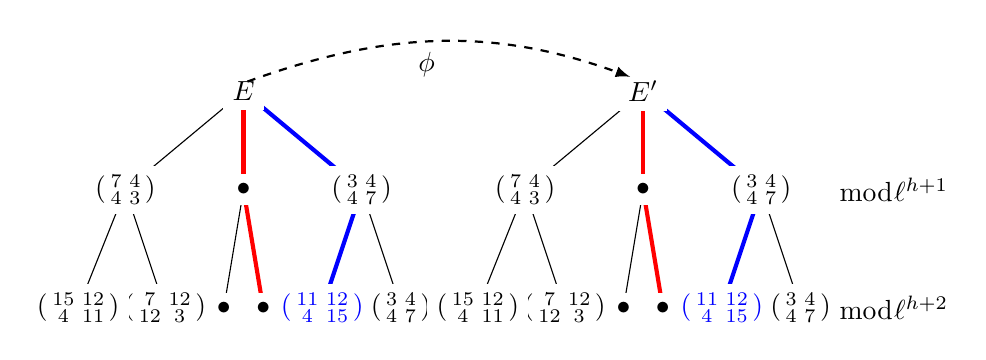
\begin{tikzpicture}[yshift=-25cm,scale=0.25]
\begin{scope}[yshift=0cm,xshift=0cm]
		\coordinate (A) at (33,-5);
		\coordinate (B) at (33,-11);
		\draw (A) node[fill=white]{$ \bmod \ell^{h+1}$};
		\draw (B) node[fill=white]{$ \bmod \ell^{h+2}$};
		\coordinate (D) at (0,0);
		\coordinate (E) at (-6,-5);
		\coordinate (F) at (6,-5);
		\coordinate (G) at (-4,-11);
		\coordinate (H) at (-8.4,-11);
		\coordinate (I) at (4,-11);
		\coordinate (J) at (8,-11);
		\coordinate (K) at (0,-5);
		\coordinate (L) at (-1,-11);
		\coordinate (M) at (1,-11);
		\draw (D) -- (E);
		\draw [line width=1.5pt,blue](D) -- (F);
		\draw [line width=1.5pt,red] (D) -- (K);
		\draw (K) -- (L);
		\draw [line width=1.5pt,red] (K) -- (M);
		\draw (E) -- (H);
		\draw (E) -- (G);
		\draw [line width=1.5pt,blue](F) -- (I);
		\draw (F) -- (J);
		\draw (D) node[fill=white]{$E$};
		\draw (K) node[fill=white]{$\bullet$};
		\draw (E) node[fill=white]{$\left( \begin{smallmatrix}7 & 4 
\\4  & 3 \end{smallmatrix} \right)$};
		\draw (F) node[fill=white]{$\left( \begin{smallmatrix}3 & 4 
\\4  & 7 \end{smallmatrix} \right) $};
		\draw (G) node[fill=white]{$\left( \begin{smallmatrix}7 & 12 
\\12  & 3 \end{smallmatrix} \right) $};
		\draw (H) node[fill=white]{$\left( \begin{smallmatrix}15 & 12 
\\4  & 11 \end{smallmatrix} \right) $};
		\draw (L) node[fill=white]{$\bullet $};
		\draw (M) node[fill=white]{$\bullet $};
		\draw (I) node[fill=white]{$ \color{blue} \left( \begin{smallmatrix}11 & 12 
\\4 & 15 \end{smallmatrix} \right) $};
		\draw (J) node[fill=white]{$\left( \begin{smallmatrix}3 & 4 
\\4  & 7 \end{smallmatrix} \right) $};
		%\coordinate (A) at (12,-5);
		%\coordinate (B) at (12,-11);
		%\draw (A) node[fill=white]{$\bmod \ell^{h+1}$};
		%\draw (B) node[fill=white]{$\bmod \ell^{h+2}$};
\end{scope}
\begin{scope}[yshift=0cm,xshift=20.3cm]
		\coordinate (D) at (0,0);
		\coordinate (E) at (-6,-5);
		\coordinate (F) at (6,-5);
		\coordinate (G) at (-4,-11);
		\coordinate (H) at (-8.4,-11);
		\coordinate (I) at (4,-11);
		\coordinate (J) at (8,-11);
		\coordinate (K) at (0,-5);
		\coordinate (L) at (-1,-11);
		\coordinate (M) at (1,-11);
		\draw (D) -- (E);
		\draw [line width=1.5pt,blue](D) -- (F);
		\draw [line width=1.5pt,red] (D) -- (K);
		\draw (K) -- (L);
		\draw [line width=1.5pt,red] (K) -- (M);
		\draw (E) -- (H);
		\draw (E) -- (G);
		\draw [line width=1.5pt,blue](F) -- (I);
		\draw (F) -- (J);
		\draw (D) node[fill=white]{$E'$};
		\draw (K) node[fill=white]{$\bullet$};
		\draw (E) node[fill=white]{$\left( \begin{smallmatrix}7 & 4 
\\4  & 3 \end{smallmatrix} \right)$};
		\draw (F) node[fill=white]{$\left( \begin{smallmatrix}3 & 4 
\\4  & 7 \end{smallmatrix} \right) $};
		\draw (G) node[fill=white]{$\left( \begin{smallmatrix}7 & 12 
\\12  & 3 \end{smallmatrix} \right) $};
		\draw (H) node[fill=white]{$\left( \begin{smallmatrix}15 & 12 
\\4  & 11 \end{smallmatrix} \right) $};
		\draw (L) node[fill=white]{$\bullet $};
		\draw (M) node[fill=white]{$\bullet $};
		\draw (I) node[fill=white]{$\color{blue} \left( \begin{smallmatrix}11 & 12 
\\4 & 15 \end{smallmatrix} \right) $};
		\draw (J) node[fill=white]{$\left( \begin{smallmatrix}3 & 4 
\\4  & 7 \end{smallmatrix} \right) $};
		%\coordinate (A) at (12,-5);
		%\coordinate (B) at (12,-11);
		%\draw (A) node[fill=white]{$\bmod \ell^{h+1}$};
		%\draw (B) node[fill=white]{$\bmod \ell^{h+2}$};
		\coordinate (A) at (-20.1,0.5);
		\coordinate (B) at (0,0.5);
		%\draw [->] (A) --(B);
		%\draw[bend right =20] (A)--(B);
		\draw[dashed,thick,-latex,shorten >=5pt] (A) to[bend left=20] node[below left] {$\phi$} (B);
\end{scope}
\end{tikzpicture}
\end{center}
%\end{figure}
%Once the image by $\phi$ of one ($\color{red} P$) of the two bases point of $E[\ell^{h+i}]$ is 
%determined, then the matrix $\pi(P,Q)$ that represents the Frobenius determines \emph{uniquely} a \emph{generator} of the
%descending $\ell^{i}$-isogenies generated by the second basis point ($\color{blue} Q$). 
Une fois que l'image par $\phi$ d'un des deux points ($\color{red} P$) de la base de la de $E[\ell^{h+i}]$ a été déterminé alors la forme de la matrice du Frobenius $\pi(P,Q)$ détermine de façon unique le générateur de la $\ell^i$-isogénie engendrée par le second point de la base
% les $\ell$-isogénies descendantes engendrées par le second point de la base.
\end{frame}


%%%%%%%%%%%%%%%%%%%%%%%%%%%%%%%%%%%%%%%%%%%%%%%%%%%%%%%%%%%%%


\begin{frame}
\begin{prop}
Il existe un entier $a$ tel que \[\mathcal{O}_K=\mathbb{Z} \left[ \frac{\pi-a}{g} \right] \quad \text{et} \quad (X-a)^2=X^2-t_{\pi}X+q \bmod g \]
\end{prop}

\end{frame}

\begin{frame}


\bluebox{Algorithme de calcul de l'anneau des endomorphismes de $E$ [Kohel '96]}{
\begin{algorithmic}[1]
\REQUIRE $d_{\pi}$ le discriminant de la courbe elliptique $E$; 
\ENSURE $\mathcal{O}$ l'anneau d'endomorphisme de $E$
\end{algorithmic}}

\begin{enumerate}
%\item Compute the prime factorization of $d_{\pi}$ and deduce from it the conductor  $g=\prod_{i=1}^j\ell_i^{t_i}$ such that $d_{\pi}=g^2d_K$ and $a$ such that $\mathcal{O}_K=\mathbb{Z} \left[ \frac{\pi-a}{g} \right] $ 
\item Factorisation de $d_{\pi}$ et calcul du conducteur 
$g=\prod_{i=1}^j\ell_i^{t_i}$ tel que $d_{\pi}=g^2d_K$ et $a$ tel que 
$\mathcal{O}_K=\mathbb{Z} \left[ \frac{\pi-a}{g} \right] $ 
\item Pour tout $\ell_i$:
\begin{enumerate}
\item Calcul de $s_i= v_{\ell_i}([\mathcal{O}:\mathbb{Z}[\pi]]) $
\end{enumerate}
\item Retourne $\mathcal{O}=\mathbb{Z}+\left( (\pi-a)/\prod_{i=1}^j\ell_i^{s_i} \right) \mathbb{Z}$
\end{enumerate}

\bluebox{Travaux précédents sur le calcul de $v_{\ell_i}([\mathcal{O}:\mathbb{Z}[\pi]]) $}{
\begin{itemize}
\item Kohel (1996) utilise les polynômes modulaires (variantes avec les polynômes de division, et les groupes de classe d'idéaux)
\item Bisson-Sutherland (2009) énumérations de relations construites à l'aide de cycles  d'isogénies
\end{itemize}
}
%Parler de Kohel (Vu dans la thèse de Mireille 1) Methode par les polynomes de division, 2) polynomes modulaires 3) Methode par les ideaux 3.a) enumeration 3.b) groupe de classe d ideaux )

%Parler de Bisson Sutherland (Utilise les cycles d'isogénies et les relations qui donnent un endomorphisme)}
\end{frame}

%%%%%%%%%%%%%%%%%%%%%%%%%%%%%%%%%%%%%%%%%%%%%%%%%%%%%%%%%%%% 


\begin{frame}
\begin{prop}
%In the Atkin case the action of the Frobenius endomorphism $\pi$ on 
%$E[\ell^{h+1}]$~is, over~$\mathbb{Z}_{\ell}$, equals to the matrix 
%\[\left ( \begin{matrix}a & b\ell^{h-e} \\ c\ell^{h-e} & d
%\end{matrix}\right ), \quad \text{with }a,d \text{ primes with }\ell, v_{\ell}(a-d)\geqslant h \]  %with $a,d $ primes with $\ell$,
%with $e$ the depth of $E$ in the volcano. Moreover 
%\begin{itemize}
%\item either $b$ and $c$ are prime with $\ell$;
%\item either one of them is prime with $\ell$ and the other has its $\ell$-adic valuation included in $ [2,2e]$.
%\end{itemize}
Dans le cas Atkin pour toute base $(P,Q)$ de $E[\ell^k]$ avec $k>h-e$ et $e$ la
profondeur de $E$ dans le volcan. L'action du Frobenius dans cette base est, à permuationt prés:
 \[\pi(P,Q)= \left ( \begin{matrix}a & b\ell^{h-e} \\ c\ell^{h-e} & d
\end{matrix}\right ) \bmod \ell^k, \quad \text{avec }a,d \text{ premier avec }\ell, v_{\ell}(a-d)\geqslant h .\]
De plus
\begin{itemize}
\item soit $b$ et $c$ sont premiers avec $\ell$;
\item soit $b$ est premier avec $\ell$ et $v_{\ell}(c) \in [2,2e]$.
\end{itemize}
\end{prop}

\begin{figure}
\begin{center}
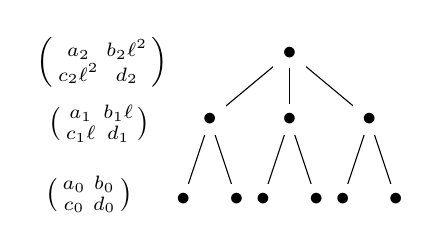
\begin{tikzpicture}[scale=0.225]
\coordinate (A) at (-2,2.5);
\coordinate (B) at (-1,6.5);
\coordinate (C) at (0,10);
\draw (A) node[left]{$\left( \begin{smallmatrix}
a_0 & b_0 \\
c_0 & d_0
\end{smallmatrix} \right) \color{black} $}; %node{$\bullet$};
\draw (B) node[left]{$ \left( \begin{smallmatrix}
a_1 & b_1\ell \\
c_1\ell & d_1
\end{smallmatrix} \right) \color{black} $}; %node{$\bullet$};
\draw (C) node[left]{$ \left( \begin{smallmatrix}
a_2 & b_2\ell^2 \\
c_2\ell^2 & d_2
\end{smallmatrix} \right) \color{black} $}; %node{$\bullet$};
\begin{scope}[yshift=10.5cm,xshift=6.3cm,scale=0.75]
		\coordinate (D) at (0,0);
		\coordinate (E) at (-6,-5);
		\coordinate (F) at (6,-5);
		\coordinate (G) at (-4,-11);
		\coordinate (H) at (-8,-11);
		\coordinate (I) at (4,-11);
		\coordinate (J) at (8,-11);
		\coordinate (K) at (0,-5);
		\coordinate (L) at (-2,-11);
		\coordinate (M) at (2,-11);
		\draw (D) -- (E);
		\draw (D) -- (F);
		\draw (D) -- (K);
		\draw (K) -- (L);
		\draw (K) -- (M);
		\draw (E) -- (H);
		\draw (E) -- (G);
		\draw (F) -- (I);
		\draw (F) -- (J);
		%\coordinate (G) at (E)++(225:3);
		\draw (D) node[fill=white]{$\bullet$};
		\draw (J) node[fill=white]{$\bullet$};
		\draw (E) node[fill=white]{$\bullet$};
		\draw (F) node[fill=white]{$\bullet$};
		\draw (G) node[fill=white]{$\bullet$};
		\draw (H) node[fill=white]{$\bullet$};
		\draw (I) node[fill=white]{$\bullet$};
		\draw (K) node[fill=white]{$\bullet$};
		\draw (L) node[fill=white]{$\bullet$};
		\draw (M) node[fill=white]{$\bullet$};
\end{scope}
\end{tikzpicture}
\end{center}
%\caption{\label{fig:atk:dif:niv:mat} Exemples de matrices du Frobenius obtenues sur les différents niveaux d'un volcan de $\ell$-isogénies}
\end{figure}
%\todo{retravailler cette slide}
%On peut donc comme dans le cas Elkies déterminer le niveau sur lequel se trouve une courbe elliptique dans le volcan d'isogénies dans le cas Atkin. 

\end{frame}

%%%%%%%%%%%%%%%%%%%%%%%%%%%%%%%%%%%%%%%%%%%%%%%%%%%%%%%%%%%%%

\begin{frame}
%A l'aide des propositions sur les formes de la matrice dans le cas Atkin et 
%Elkies on peut savoir à quel niveau du volcan se trouve une courbe elliptique.
%
% 
%Faire une slide qui parle de ça 
%Il faut juste dire comment l'on distingue un cas Atkin d'un cas Elkies...
%Faire une estimation à la louche
\bluebox{Algorithme de calcul de l'anneau des endomorphismes de $E$ [Kohel '96]}{
\begin{algorithmic}[1]
\REQUIRE $d_{\pi}$ le discriminant de la courbe elliptique $E$; 
\ENSURE $\mathcal{O}$ l'anneau d'endomorphisme de $E$
\end{algorithmic}}

\bluebox{}{\textbf{Fait:} Pour $\langle P, R \rangle = E[\ell_i^{r_i+1}]$ avec $r_i=\lfloor v_{\ell_i}(d_{\pi})/2 \rfloor $ à partir de $\pi(P,R)$ nous déduisons $v_{\ell_i}([\mathcal{O}:\mathbb{Z}[\pi]])$.}

\begin{enumerate}
\item \`A partir de la factorisation de $d_{\pi}$ calcul du conducteur $g=\prod_{i=1}^j\ell_i^{t_i}$ de $\mathbb{Z}[\pi]$ et $a$ tel que $\mathcal{O}_K=\mathbb{Z} \left[ \frac{\pi-a}{g} \right] $ 
\item Pour tout $\ell_i$:
\begin{enumerate}
\item Calcul de $\langle P , Q \rangle = E[\ell_i^{r_i+1}]$
\medskip
\item Détermination à partir de $d_{\pi}$ si $\ell_i$ est un nombre premier de Atkin ou de Elkies 
\medskip 
\item Détermination de $s_i=v_{\ell_i}([\mathcal{O}:\mathbb{Z}[\pi]])$ à partir de  $\pi(P,Q)$
\end{enumerate}
\item Retourne $\mathcal{O}=\mathbb{Z} + \left( (\pi-a)/ \prod_{i=1}^j\ell_i^{s_i} \right) \mathbb{Z}$
\end{enumerate}
\end{frame}

%%%%%%%%%%%%%%%%%%%%%%%%%%%%%%%%%%%%%%%%%%%%%%%%%%%%%%%%%%%%%

\begin{frame}
\frametitle{Comparaison avec le cas Elkies}
\begin{figure}
\begin{center}

\begin{tikzpicture}[scale=0.290]

\begin{scope}[yshift=10cm]
	\begin{scope}[xshift=4.3cm]
		\coordinate (A) at (-3,0);
		\coordinate (B) at (3,0);
		\coordinate (C) at (270:1.2);
		\draw[-] (A.center) to[bend right=25] (C.center);
		\draw[-,dashed] (A.center) to[bend left=40] (B.center);
		%\draw[-] (A.center) to[bend right=40] (B.center);
		\draw[line width=2.25pt,red] (B.center) to[bend left=25] (C.center);
		%\draw[-,dashed] (B.center) to[bend right] (D.center);
		%\draw[line width=2.5pt,red,->] (A.center) to[bend right=20] (C.center);
			\begin{scope}[xshift=-3cm]% sous volcan de gauche
			\coordinate (A) at (0,0);
			\coordinate (C) at (270:4.2);
			\coordinate (CA) at (265:7.5);
			\coordinate (CB) at (275:7.5);
			\draw (C)--(CA);
			\draw (C)--(CB);
			\draw (A)--(C);
			\draw (CA) node[fill=white]{$\bullet$};
			\draw (CB) node[fill=white]{$\bullet$};
			\draw (A) node[fill=white]{$\bullet$};
			\draw (C) node[fill=white]{$\bullet$};
			\end{scope}
			\begin{scope}[xshift=3cm]% sous volcan de droite
			\coordinate (A) at (0,0);
			\coordinate (C) at (270:4.2);
			\coordinate (CA) at (265:7.5);
			\coordinate (CB) at (275:7.5);
			\draw [line width=1.5pt,red] (C)--(A);
			\draw (C)--(CB);
			\draw (C)--(CA);
			\draw (CA) node[fill=white]{$\bullet$};
			\draw (CB) node[fill=white]{$\bullet$};
			\draw (A) node[fill=white]{$\bullet$};
			\draw (C) node[fill=white]{$\bullet$};
			\end{scope}
			\begin{scope}[yshift=-1.2cm] %sous volcan du bas
			\coordinate (A) at (0,0);
			\coordinate (C) at (270:4.2);
			\coordinate (CA) at (265:7.5);
			\coordinate (CB) at (275:7.5);
			\draw (C)--(CA);
			\draw (C)--(CB);
			\draw [line width=1.5pt,blue] (A)--(C);
			%\draw (CA) node[fill=white]{$\bullet$};
			\coordinate (CAB) at (260:8.5);
			\coordinate (CBB) at (280:8.5);
			\draw (CAB) node {$ \left( \begin{smallmatrix}
					7 & 4 \\
					0 & 3
					\end{smallmatrix} \right) $};
			%\draw (CB) node[fill=white]{$\bullet$};
			\draw (CBB) node{$ \left( \begin{smallmatrix}
					7 & 4 \\
					0 & 3
					\end{smallmatrix} \right) $};
			%c est de la triche ce sont les seules matrices possibles...
			%\draw (A) node{$\bullet$};
			\only<1>{
			\draw [line width=1.5pt,blue] (C)--(CA);
			\draw (CAB) node {$ \color{blue} \left( \begin{smallmatrix}
					7 & 4 \\
					0 & 3
					\end{smallmatrix} \right) $};
			}
			\only<2>{
			\draw [line width=1.5pt,blue] (C)--(CB);
			\draw (CBB) node{$ \color{blue} \left( \begin{smallmatrix}
					7 & 4 \\
					0 & 3
					\end{smallmatrix} \right) $};
			}			
			\draw (C) node[fill=white]{$\bullet$};
			\draw (A) node[fill=white]{$E$};
			
			
			%(C) node[left]{$\mathcal{O}$} node{$\bullet$};			
			
			\end{scope}
			\coordinate (F) at (5,0);
			\coordinate (G) at (5,-7);
			\draw[dashed,<-] (F)--(G) node[midway,right]{$h$};
	\end{scope}
\end{scope}

%faire des fleches courbees avec les indices \ell et \ell^2

\end{tikzpicture}
\end{center}

\caption{\label{fig:elk:dif:niv:mat} Matrices du Frobenius possibles pour une base de $E[8]$ avec le premier vecteur de la base ($\color{red} P$) fixé et le second ($\color{blue} R$) qui engendre la $4$-isogénie descendante}
\end{figure}
\end{frame}

%%%%%%%%%%%%%%%%%%%%%%%%%%%%%%%%%%%%%%%%%%%%%%%%%%%%%%%

\begin{frame}
\frametitle{Un algorithme de Couveignes $\ell$-adique dans le cas Atkin}
%\begin{figure}
\begin{center}
\begin{tikzpicture}[yshift=-25cm,scale=0.25]
\begin{scope}[yshift=0cm,xshift=0cm]
		\coordinate (D) at (0,0);
		\coordinate (E) at (-6,-5);
		\coordinate (F) at (6,-5);
		\coordinate (G) at (-4,-11);
		\coordinate (H) at (-8.4,-11);
		\coordinate (I) at (4,-11);
		\coordinate (J) at (8,-11);
		\coordinate (K) at (0,-5);
		\coordinate (L) at (-1,-11);
		\coordinate (M) at (1,-11);
		\only<1>{
		\draw [gray!25] (D) -- (E);
		\draw [gray!25] (K) -- (L);
		\draw [line width=1.5pt,blue!25](D) -- (F);
		\draw [line width=1.5pt,red!25] (D) -- (K);
		\draw [line width=1.5pt,red!25] (K) -- (M);
		\draw [gray!25] (E) -- (H);
		\draw [gray!25] (E) -- (G);
		\draw [line width=1.5pt,blue!25](F) -- (I);
		\draw [gray!25] (F) -- (J);
		\draw (K) node[fill=white]{$\color{gray!25}{ \bullet}$};
		\draw (E) node[fill=white]{$\color{black!25} \left( \begin{smallmatrix}0 & 1 
\\1  & 1 \end{smallmatrix} \right)$};
		\draw (F) node[fill=white]{$\color{black!25} \left( \begin{smallmatrix}1 & 1 
\\1  & 0 \end{smallmatrix} \right) $};
		\draw (G) node[fill=white]{$\color{black!25} \left( \begin{smallmatrix}0 & 1 
\\3  & 3 \end{smallmatrix} \right) $};
		\draw (H) node[fill=white]{$\color{black!25} \left( \begin{smallmatrix}2 & 1 
\\1  & 1 \end{smallmatrix} \right) $};
		\draw (L) node[fill=white]{$\color{gray!25}{ \bullet }$};
		\draw (M) node[fill=white]{$\color{gray!25}{ \bullet }$};
		\draw (I) node[fill=white]{$ \color{blue!25} \left( \begin{smallmatrix}3 & 1 
\\3 & 0 \end{smallmatrix} \right) $};
		\draw (J) node[fill=white]{$\color{black!25} \left( \begin{smallmatrix}1 & 1 
\\1  & 2 \end{smallmatrix} \right) $};
		}
		\only<2>{
		\draw (D) -- (E);
		\draw (K) -- (L);
		\draw [line width=1.5pt,blue](D) -- (F);
		\draw [line width=1.5pt,red] (D) -- (K);
		\draw [line width=1.5pt,red] (K) -- (M);
		\draw (E) -- (H);
		\draw (E) -- (G);
		\draw [line width=1.5pt,blue](F) -- (I);
		\draw (F) -- (J);
		\draw (K) node[fill=white]{$\bullet$};
		\draw (E) node[fill=white]{$\left( \begin{smallmatrix}0 & 1 
\\1  & 1 \end{smallmatrix} \right)$};
		\draw (F) node[fill=white]{$\left( \begin{smallmatrix}1 & 1 
\\1  & 0 \end{smallmatrix} \right) $};
		\draw (G) node[fill=white]{$\left( \begin{smallmatrix}0 & 1 
\\3  & 3 \end{smallmatrix} \right) $};
		\draw (H) node[fill=white]{$\left( \begin{smallmatrix}2 & 1 
\\1  & 1 \end{smallmatrix} \right) $};
		\draw (L) node[fill=white]{$\bullet $};
		\draw (M) node[fill=white]{$\bullet $};
		\draw (I) node[fill=white]{$ \color{blue} \left( \begin{smallmatrix}3 & 1 
\\3 & 0 \end{smallmatrix} \right) $};
		\draw (J) node[fill=white]{$\left( \begin{smallmatrix}1 & 1 
\\1  & 2 \end{smallmatrix} \right) $};}
		\draw (D) node[fill=white]{$E$};
		%\coordinate (A) at (12,-5);
		%\coordinate (B) at (12,-11);
		%\draw (A) node[fill=white]{$\bmod \ell^{h+1}$};
		%\draw (B) node[fill=white]{$\bmod \ell^{h+2}$};
\end{scope}
\begin{scope}[yshift=0cm,xshift=20.3cm]
		\coordinate (A) at (33,-5);
		\coordinate (B) at (33,-11);
		\draw (A) node[fill=white]{$ \bmod \ell^{1}$};
		\draw (B) node[fill=white]{$ \bmod \ell^{2}$};
		\coordinate (D) at (0,0);
		\coordinate (E) at (-6,-5);
		\coordinate (F) at (6,-5);
		\coordinate (G) at (-4,-11);
		\coordinate (H) at (-8.4,-11);
		\coordinate (I) at (4,-11);
		\coordinate (J) at (8,-11);
		\coordinate (K) at (0,-5);
		\coordinate (L) at (-1,-11);
		\coordinate (M) at (1,-11);
		\only<1>{
		\draw [gray!25] (D) -- (E);
		\draw [gray!25] (K) -- (L);
		\draw [line width=1.5pt,blue!25](D) -- (F);
		\draw [line width=1.5pt,red!25] (D) -- (K);
		\draw [line width=1.5pt,red!25] (K) -- (M);
		\draw [gray!25] (E) -- (H);
		\draw [gray!25] (E) -- (G);
		\draw [line width=1.5pt,blue!25](F) -- (I);
		\draw [gray!25] (F) -- (J);
		\draw (K) node[fill=white]{$\color{gray!25}{ \bullet}$};
		\draw (E) node[fill=white]{$\color{black!25} \left( \begin{smallmatrix}0 & 1 
\\1  & 1 \end{smallmatrix} \right)$};
		\draw (F) node[fill=white]{$\color{black!25} \left( \begin{smallmatrix}1 & 1 
\\1  & 0 \end{smallmatrix} \right) $};
		\draw (G) node[fill=white]{$\color{black!25} \left( \begin{smallmatrix}0 & 1 
\\3  & 3 \end{smallmatrix} \right) $};
		\draw (H) node[fill=white]{$\color{black!25} \left( \begin{smallmatrix}2 & 1 
\\1  & 1 \end{smallmatrix} \right) $};
		\draw (L) node[fill=white]{$\color{gray!25}{ \bullet }$};
		\draw (M) node[fill=white]{$\color{gray!25}{ \bullet }$};
		\draw (I) node[fill=white]{$ \color{blue!25} \left( \begin{smallmatrix}3 & 1 
\\3 & 0 \end{smallmatrix} \right) $};
		\draw (J) node[fill=white]{$\color{black!25} \left( \begin{smallmatrix}1 & 1 
\\1  & 2 \end{smallmatrix} \right) $};
		}
		\only<2>{
		\draw (D) -- (E);
		\draw (K) -- (L);
		\draw [line width=1.5pt,blue](D) -- (F);
		\draw [line width=1.5pt,red] (D) -- (K);
		\draw [line width=1.5pt,red] (K) -- (M);
		\draw (E) -- (H);
		\draw (E) -- (G);
		\draw [line width=1.5pt,blue](F) -- (I);
		\draw (F) -- (J);
		\draw (K) node[fill=white]{$\bullet$};
		\draw (E) node[fill=white]{$\left( \begin{smallmatrix}0 & 1 
\\1  & 1 \end{smallmatrix} \right)$};
		\draw (F) node[fill=white]{$\left( \begin{smallmatrix}1 & 1 
\\1  & 0 \end{smallmatrix} \right) $};
		\draw (G) node[fill=white]{$\left( \begin{smallmatrix}0 & 1 
\\3  & 3 \end{smallmatrix} \right) $};
		\draw (H) node[fill=white]{$\left( \begin{smallmatrix}2 & 1 
\\1  & 1 \end{smallmatrix} \right) $};
		\draw (L) node[fill=white]{$\bullet $};
		\draw (M) node[fill=white]{$\bullet $};
		\draw (I) node[fill=white]{$ \color{blue} \left( \begin{smallmatrix}3 & 1 
\\3 & 0 \end{smallmatrix} \right) $};
		\draw (J) node[fill=white]{$\left( \begin{smallmatrix}1 & 1 
\\1  & 2 \end{smallmatrix} \right) $};}
		\draw (D) node[fill=white]{$E$};
		%\coordinate (A) at (12,-5);
		%\coordinate (B) at (12,-11);
		%\draw (A) node[fill=white]{$\bmod \ell^{h+1}$};
		%\draw (B) node[fill=white]{$\bmod \ell^{h+2}$};
		\draw (D) node[fill=white]{$E'$};
		\coordinate (A) at (-20.1,0.5);
		\coordinate (B) at (0,0.5);
		%\draw [->] (A) --(B);
		%\draw[bend right =20] (A)--(B);
		\draw[dashed,thick,-latex,shorten >=5pt] (A) to[bend left=20] node[below left] {$\phi$} (B);
\end{scope}
\end{tikzpicture}
\end{center}
%\end{figure}
%Once the image by $\phi$ of one ($\color{red} P$) of the two bases point of $E[\ell^{h+i}]$ is 
%determined, then the matrix $\pi(P,Q)$ that represents the Frobenius determines \emph{uniquely} a \emph{generator} of the
%descending $\ell^{i}$-isogenies generated by the second basis point ($\color{blue} Q$). 
\only<2>{Une fois que l'image par $\phi$ d'un des deux points ($\color{red} P$) de la 
base $\langle P, Q \rangle$ de $E[\ell^{2}]$ a été déterminée alors la forme de
la matrice du Frobenius dans une telle base notée $\pi(P,Q)$ détermine de façon
unique le générateur de la $\ell^2$-isogénie engendrée par le second point 
$(Q)$ de la base.}
% les $\ell$-isogénies descendantes engendrées par le second point de la base.
\end{frame}

%%%%%%%%%%%%%%%%%%%%%%%%%%%%%%%%%%%%%%%%%%%%%%%%%%%%%%%

\begin{frame}
\frametitle{Volcan et tour d'extensions}

\begin{figure}
\begin{center}

\begin{tikzpicture}[scale=0.55]
\coordinate (A) at (-2,1.5);	
\coordinate (B) at (-2,5);
\coordinate (C) at (-2,10);
\coordinate (D) at (-2,7.5);
\draw [gray!30] (D)--(C);
\draw [gray!30] (C)--(B);
\draw [gray!30] (A)--(B);
\only<2->{
\draw (D)--(C);}
\only<4>{
\draw (A)--(B);}
\only<3->{
\draw (B)--(D);}
\draw (C) node[left]{$\mathbb{F}_q$} node{$\bullet$};
\draw (A) node[left,gray!30]{$\mathsf{F}_3$} node[gray!30]{$\bullet$};
\draw (B) node[left,gray!30]{$\mathsf{F}_2$} node[gray!30]{$\bullet$};
\draw (D) node[left,gray!30]{$\mathsf{F}_1$} node[gray!30]{$\bullet$};
\only<2->{
\draw (D) node[left]{$\mathsf{F}_1$} node{$\bullet$};}
\only<3->{
\draw (B) node[left]{$\mathsf{F}_2$} node{$\bullet$};}
\only<4->{
\draw (A) node[left]{$\mathsf{F}_3$} node{$\bullet$};}

%\draw (CZ)--(BZ)[dashed]  node[midway,left] {$\ell$};
%\draw (BZ2)--(AZ)[dashed]  node[midway,left] {$\ell$};
\begin{scope}[yshift=10cm,xshift=6cm]
		\node (A) at (-4,0) {$  \bullet $};
		\node (B) at (4,0) {$   \bullet$};
		\node (C) at (270:1.2) {$ \bullet \color{black}$};
		\node (D) at (90:1.5) {};
		%\draw[-] (A.center) to[bend right=25] (C.center);
		\draw[-] (A.center) to[bend left=40] (B.center);
		%\draw[-] (B.center) to[bend left=25] (C.center);
		%\draw[-,dashed] (B.center) to[bend right] (D.center);
		\draw[-] (A.center) to[bend right=30] (B.center);
		\draw (A) node{$  \bullet $};
		\draw (B) node{$  \bullet $};
		\draw (C) node{$  \bullet $};
		%\draw[line width=2.5pt,red,->] (A.center) to[bend right=20] (C.center);
			\begin{scope}[xshift=-4cm]% sous volcan de gauche
			\coordinate (A) at (0,0);
			\coordinate (C) at (0,-3);
			\coordinate (CA) at (1,-6);
			\coordinate (CB) at (-1,-6);
			\coordinate (CAA) at (1.4,-9);
			\coordinate (CAB) at (0.6,-9);
			\coordinate (CBA) at (-0.6,-9);
			\coordinate (CBB) at (-1.4,-9);
			\only<1-2>{
			\draw [dashed,gray!30] (C)--(CA);
			\draw [dashed,gray!30] (C)--(CB);}
			\only<3->{
			\draw (C)--(CA);
			\draw (C)--(CB);}
			\only<1>{
			\draw [dashed,gray!30] (A)--(C);
			\draw (C) node[fill=white]{$\bullet$};
			\draw (A) node[fill=white] {$\bullet$};
			\draw (C) node[gray!30]{$\bullet$};}
			\only<2->{
			\draw (A)--(C);
			\draw (C) node[fill=white]{$\bullet$};
			\draw (A) node[fill=white]{$\bullet$};}
			\only<1-3>{
			\draw [dashed,gray!30] (CA)--(CAA);
			\draw [dashed,gray!30] (CA)--(CAB);
			\draw [dashed,gray!30] (CB)--(CBA);
			\draw [dashed,gray!30] (CB)--(CBB);}
			\only<4>{
			\draw (CA)--(CAA);
			\draw (CA)--(CAB);
			\draw (CB)--(CBA);
			\draw (CB)--(CBB);}
			\only<1-2>{
			\draw (CA) node[fill=white]{$\bullet$};
			\draw (CA) node[gray!30]{$\bullet$};
			\draw (CB) node[fill=white]{$\bullet$};
			\draw (CB) node[gray!30]{$\bullet$};}
			\only<3->{
			\draw (CA) node[fill=white]{$\bullet$};
			\draw (CB) node[fill=white]{$\bullet$};}
			\only<4>{
			\draw (CAA) node[fill=white]{$\bullet$};
			\draw (CAB) node[fill=white]{$\bullet$};
			\draw (CBA) node[fill=white]{$\bullet$};
			\draw (CBB) node[fill=white]{$\bullet$};}
			\only<1-3>{
			\draw (CAA) node[fill=white]{$\bullet$};
			\draw (CAA) node[gray!30]{$\bullet$};
			\draw (CAB) node[fill=white]{$\bullet$};
			\draw (CAB) node[gray!30]{$\bullet$};
			\draw (CBA) node[fill=white]{$\bullet$};
			\draw (CBA) node[gray!30]{$\bullet$};
			\draw (CBB) node[fill=white]{$\bullet$};
			\draw (CBB) node[gray!30]{$\bullet$};}
			\end{scope}
			\begin{scope}[xshift=4cm]% sous volcan de droite
			\coordinate (A) at (0,0);
			\coordinate (C) at (0,-3);
			\coordinate (CA) at (1,-6);
			\coordinate (CB) at (-1,-6);
			\coordinate (CAA) at (1.4,-9);
			\coordinate (CAB) at (0.6,-9);
			\coordinate (CBA) at (-0.6,-9);
			\coordinate (CBB) at (-1.4,-9);
			\only<1-2>{
			\draw [dashed,gray!30] (C)--(CA);
			\draw [dashed,gray!30] (C)--(CB);}
			\only<3->{
			\draw (C)--(CA);
			\draw (C)--(CB);}
			\only<1>{
			\draw [dashed,gray!30] (A)--(C);
			\draw (C) node[fill=white]{$\bullet$};
			\draw (A) node[fill=white] {$\bullet$};
			\draw (C) node[gray!30]{$\bullet$};}
			\only<2->{
			\draw (A)--(C);
			\draw (C) node[fill=white]{$\bullet$};
			\draw (A) node[fill=white]{$\bullet$};}
			\only<1-3>{
			\draw [dashed,gray!30] (CA)--(CAA);
			\draw [dashed,gray!30] (CA)--(CAB);
			\draw [dashed,gray!30] (CB)--(CBA);
			\draw [dashed,gray!30] (CB)--(CBB);}
			\only<4>{
			\draw (CA)--(CAA);
			\draw (CA)--(CAB);
			\draw (CB)--(CBA);
			\draw (CB)--(CBB);}
			\only<1-2>{
			\draw (CA) node[fill=white]{$\bullet$};
			\draw (CA) node[gray!30]{$\bullet$};
			\draw (CB) node[fill=white]{$\bullet$};
			\draw (CB) node[gray!30]{$\bullet$};}
			\only<3->{
			\draw (CA) node[fill=white]{$\bullet$};
			\draw (CB) node[fill=white]{$\bullet$};}
			\only<4>{
			\draw (CAA) node[fill=white]{$\bullet$};
			\draw (CAB) node[fill=white]{$\bullet$};
			\draw (CBA) node[fill=white]{$\bullet$};
			\draw (CBB) node[fill=white]{$\bullet$};}
			\only<1-3>{
			\draw (CAA) node[fill=white]{$\bullet$};
			\draw (CAA) node[gray!30]{$\bullet$};
			\draw (CAB) node[fill=white]{$\bullet$};
			\draw (CAB) node[gray!30]{$\bullet$};
			\draw (CBA) node[fill=white]{$\bullet$};
			\draw (CBA) node[gray!30]{$\bullet$};
			\draw (CBB) node[fill=white]{$\bullet$};
			\draw (CBB) node[gray!30]{$\bullet$};}
			\end{scope}
			\begin{scope}[yshift=-1.2cm] %sous volcan du bas
			\coordinate (A) at (0,0);
			\coordinate (C) at (0,-3);
			\coordinate (CA) at (1,-6);
			\coordinate (CB) at (-1,-6);
			\coordinate (CAA) at (1.4,-9);
			\coordinate (CAB) at (0.6,-9);
			\coordinate (CBA) at (-0.6,-9);
			\coordinate (CBB) at (-1.4,-9);
			\only<1-2>{
			\draw [dashed,gray!30] (C)--(CA);
			\draw [dashed,gray!30] (C)--(CB);}
			\only<3->{
			\draw (C)--(CA);
			\draw (C)--(CB);}
			\only<1>{
			\draw [dashed,gray!30] (A)--(C);
			\draw (C) node[fill=white]{$\bullet$};
			\draw (A) node[fill=white] {$\bullet$};
			\draw (C) node[gray!30]{$\bullet$};}
			\only<2->{
			\draw (A)--(C);
			\draw (C) node[fill=white]{$\bullet$};
			\draw (A) node[fill=white]{$\bullet$};}
			\only<1-3>{
			\draw [dashed,gray!30] (CA)--(CAA);
			\draw [dashed,gray!30] (CA)--(CAB);
			\draw [dashed,gray!30] (CB)--(CBA);
			\draw [dashed,gray!30] (CB)--(CBB);}
			\only<4>{
			\draw (CA)--(CAA);
			\draw (CA)--(CAB);
			\draw (CB)--(CBA);
			\draw (CB)--(CBB);}
			\only<1-2>{
			\draw (CA) node[fill=white]{$\bullet$};
			\draw (CA) node[gray!30]{$\bullet$};
			\draw (CB) node[fill=white]{$\bullet$};
			\draw (CB) node[gray!30]{$\bullet$};}
			\only<3->{
			\draw (CA) node[fill=white]{$\bullet$};
			\draw (CB) node[fill=white]{$\bullet$};}
			\only<4>{
			\draw (CAA) node[fill=white]{$\bullet$};
			\draw (CAB) node[fill=white]{$\bullet$};
			\draw (CBA) node[fill=white]{$\bullet$};
			\draw (CBB) node[fill=white]{$\bullet$};}
			\only<1-3>{
			\draw (CAA) node[fill=white]{$\bullet$};
			\draw (CAA) node[gray!30]{$\bullet$};
			\draw (CAB) node[fill=white]{$\bullet$};
			\draw (CAB) node[gray!30]{$\bullet$};
			\draw (CBA) node[fill=white]{$\bullet$};
			\draw (CBA) node[gray!30]{$\bullet$};
			\draw (CBB) node[fill=white]{$\bullet$};
			\draw (CBB) node[gray!30]{$\bullet$};}
			\end{scope}
\end{scope}

%faire des fleches courbees avec les indices \ell et \ell^2


\end{tikzpicture}
\end{center}		
\end{figure}
\end{frame}

%%%%%%%%%%%%%%%%%%%%%%%%%%%%%%%%%%%%%%%%%%%%%%%%%%%%%%%%%%%%%%%%%%%%%%%%

\backupend
\end{document}


%%%%%%%%%%%%%%%%%%%%%%%%%%%%%%%%%%%%%%%%%%%%%%%%%%%%%%%%%%

\begin{frame}
%Parler de la représentation univariée et bivariée, dire que les calculs sont toujours plus rapide en univariée, montrer le passage d'une représentation bivariée à univariée. Dire que l'on peut ajouter des étages à la volée. Mentionner que l'on a des bonnes complexités pour le Frobenius en particulier.

\bluebox{Représentation univariée}
{
Un élément de $F_k$ est dit sous forme univariée si il est écrit à l'aide d'un polynôme $G \in \mathbb{F}_q[X]$ de degré inférieur à $d_1\ell^{k-1}$, avec $d_1=[\mathsf{F}_1:\mathbb{F}_q]$, évalué en l'élément primitif $x_k$ de $F_k$.
}

\begin{exe}
Soit $\mathbb{F}_q, \mathsf{F}_1, \mathsf{F}_2, \cdots, \mathsf{F}_k$ une tour d'extensions $5$-adiques telle que $\mathbb{F}_q \cong \mathsf{F}_1$ (id est $d_1=1$), soit $x_4$ un élément primitif de $\mathsf{F}_4$ alors une représentation univariée d'un élément $\beta \in \mathsf{F}_4$ est:
\begin{equation*}
 \beta_0 + \beta_1 x_4+ \cdots +\beta_{5k}x_4^{5k} + \beta_{5k+1}x_4^{5k+1}+ \cdots +\beta_{5k+4}x_4^{5k+4}+ \cdots + \beta_{124}x_4^{124}
\end{equation*}
\end{exe}
\end{frame}

%%%%%%%%%%%%%%%%%%%%%%%%%%%%%%%%%%%%%%%%%%%%%%%%%%%%%%%%%%%%%%%%%

\begin{frame}
\bluebox{Représentation bivariée}
{
Un élément de $\mathsf{F}_k$ est dit sous forme bivariée si il est écrit à l'aide des éléments primitifs $x_k$ de $\mathsf{F}_k$ et $x_{k-1}$ de $\mathsf{F}_{k-1}$ sous la forme: 
\begin{equation*}
 G_0(x_k)+G_1(x_{k-1})+x_kG_2(x_{k-1})+ \cdots x_k^{\ell-1}G_{\ell}(x_{k-1})
\end{equation*}
avec $G_i \in \mathbb{F}_q[X]$ de degré inférieur à $d_1\ell^{k-2}$ avec $d_1=[\mathsf{F}_1:\mathbb{F}_q]$ pour $i>0$ et $G_0$ de degré inférieur à $\ell$.
}
\begin{exe}
Ainsi $\beta \in \mathsf{F}_4$ a la représentation bivariée suivante:
\begin{equation*}
  \beta_0 + \beta_1 x_4+ \cdots + x_3^{k}(\beta_{5k}+\beta_{5k+1} x_4 + \beta_{5k+2} x_4^2 + \beta_{5k+3} x_4^3 + \beta_{5k+4}x_3^4)+ \cdots + \beta_{124}x_3^{24}x_4^{4}.
 \end{equation*} 
en se servant du fait que $x_4^5=x_3$.
\end{exe}
\end{frame}

%%%%%%%%%%%%%%%%%%%%%%%%%%%%%%%%%%%%%%%%%%%%%%%%%%%%%%%%%%%%

\begin{frame}
\bluebox{Changement de représentation univariée, bivariée}
{Celui-ci consiste à passer d'une écriture à une autre.
\begin{equation*}
\begin{alignedat}{1}
 G(x_k) &= G_0(x_k)+ G_1(x_k^\ell)+x_kG_2(x_k^\ell)+ \cdots + x_k^{\ell-1} G_{\ell}(x_k^{\ell})\\
&= G_0(x_k)+G_1(x_{k-1})+x_kG_2(x_{k-1})+ \cdots x_k^{\ell-1}G_{\ell}(x_{k-1})
\end{alignedat}
\end{equation*}
Celui-ci n'a pas de coût algébrique.}

\begin{exe}
Soit $\alpha \in \mathsf{F}_4$ qui s'écrit dans la base univariée de $\mathsf{F}_4$:
\begin{equation}
\label{eq:exe:mon}
\alpha_0 + \alpha_5x_4^5+ \alpha_{10}x_4^{10} + \alpha_{15}x_4^{15} + \cdots + \alpha_{5k}x_4^{5k} + \cdots + \alpha_{120}x_4^{120} 
\end{equation} 
alors $\alpha$ s'écrit de la façon suivante dans la base bivariée de $\mathsf{F}_4$:
\begin{equation}
\label{eq:exe:biv}
\alpha_0 + \alpha_5x_3^1+ \alpha_{10}x_3^{2} + \alpha_{15}x_3^{3} + \cdots + \alpha_{5k}x_3^{k} + \cdots + \alpha_{120}x_3^{24}. 
\end{equation} 
 Ainsi $\alpha \in \mathsf{F}_3$. Le passage de la représentation de $\alpha$ de \eqref{eq:exe:mon} à \eqref{eq:exe:biv} correspond à une \emph{descente}, l'opération inverse est elle un \emph{relèvement}.
\end{exe}

%Cela permet notamment d'ajouter sans coût supplémentaire des étages à la tour.

\end{frame}
%%%%%%%%%%%%%%%%%%%%%%%%%%%%%%%%%%%%%%%%%%%%%%%%%%%%%%%%%%%%

\begin{frame}
\frametitle{Motivation}
How to communicate securely on a channel that is not ?
%mettre une image de communication entre deux personnes
\only<1-1>{
\begin{center}
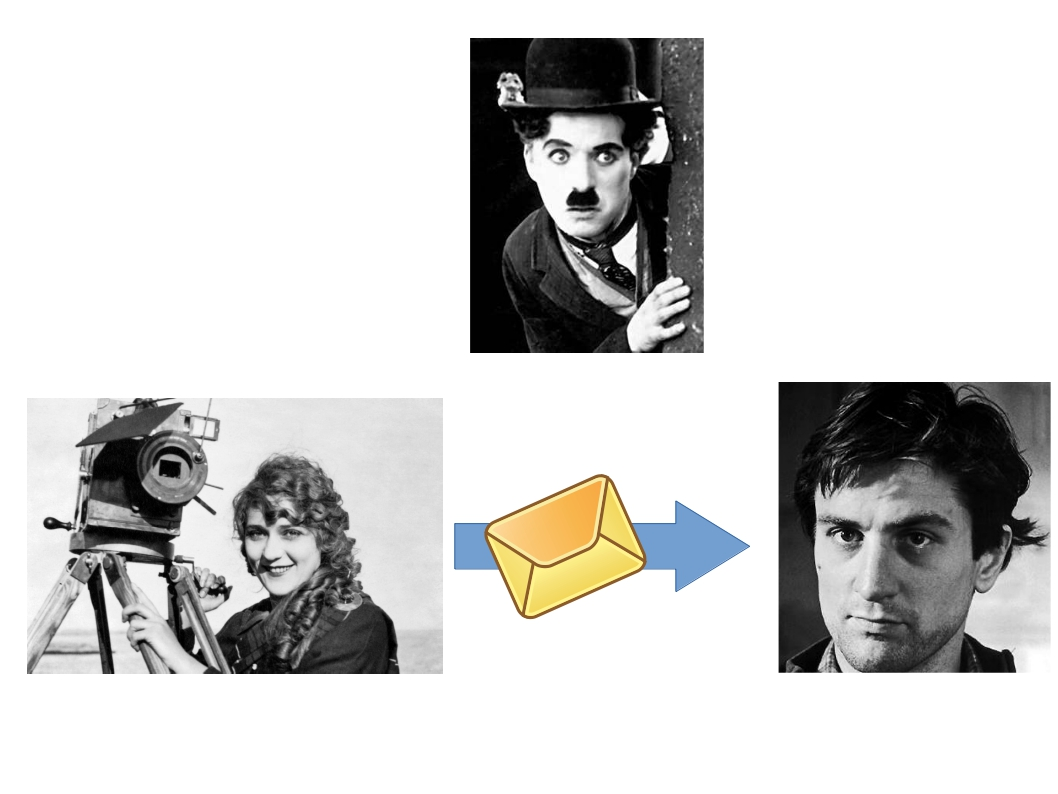
\includegraphics[scale=0.30]{Images/communication_Alice_Bob.jpg} 
\end{center}
}
\only<2-2>{
\begin{center}
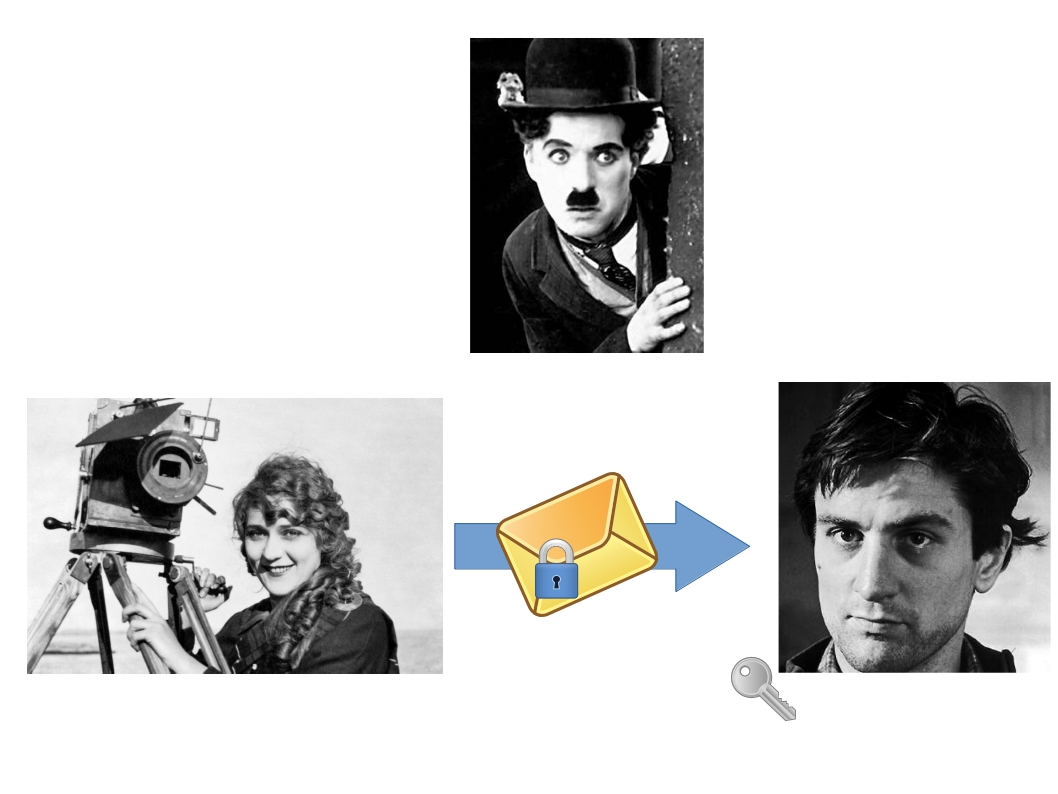
\includegraphics[scale=0.30]{Images/communication_Alice_Bob_chiffre.jpg} 
\end{center}
}
\only<3-3>{
\begin{center}
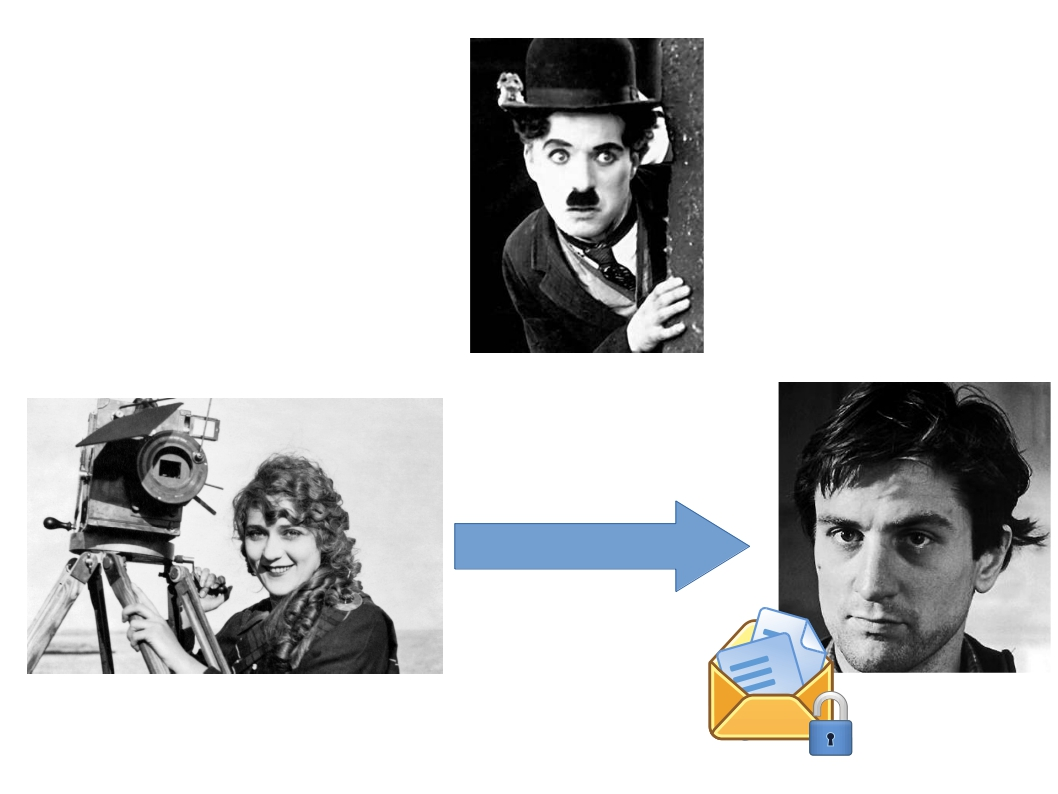
\includegraphics[scale=0.30]{Images/communication_Alice_Bob_dechiffre.jpg} 
\end{center}
}
%Dire que cette protection se fait a l aide d unn probleme mathematique juge  difficile
%parler de canaux non-sécurisés...
%\bluebox{Cryptography}
%{It is a way to communicate in a secured way on a channel that is not}

% parle de cryptographie symmétrique la clé de chiffrement et de déchiffrement sont identiques, et asymmétriques la clé de chiffrement et de déchiffrement sont différentes...
\end{frame}

%Faire une slide disant que l'on a pas la correspondance entre les différentes isogénies descendantes et ensuite embrayer sur les isogénies horizontales...
%De plus on est pas capable de distinguer les isogénies descendantes.

%\begin{prop}
%\label{pro:etu:atk:elk}
%
%Soit $\langle P ,R \rangle = E[\ell^{h-e+1}]$ pour $E$ située au niveau $h-e$ 
%du volcan. Alors pour toute $\ell$-isogénie $\psi$ descendante de domaine $E$ 
%il existe $R'$ tel que $\ker(\psi)=\langle [\ell^{h-e}]R' \rangle$, $\langle P,R' 
%\rangle = E[\ell^{h-e+1}]$ et $ \pi(P,R)= \pi(P,R') $
%\end{prop}
%\pause
%Le Frobenius ne permet pas de distinguer les isogénies descendantes.


